%!TEX root = main.tex
% \resetcounters
\chapter{Linear Quadratic Robust Model Predictive Control}\label{ch:MPC:sec:quadratic:MPC}
%
%
In most cases robust model predictive control problems can not be solved algorithmically unless a particular structure is assumed.
%
A common case for which we are able to determine the exact solution numerically is the setup where the cost is quadratic and the constraints are linear.
%
Again, many methods for quadratic nominal model predictive control problems can be extended to the robust case.
%
The general closed-loop problem formulation~\eqref{ch:concepts:general:rmpc:problem:formulation} in the quadratic case takes the form of
%
\begin{subequations}\label{ch:quad:MPC:unspecific:constraints}
\begin{equation}
	J_m^\ast(x) = \min_{u} \max_{w} \frac{1}{2}\left(x^T Q x + u^TRu - \gamma^2 w^T w\right) + J_{m-1}^\ast(x^+)
\end{equation}
%
subject to
%
\begin{equation}
	x^+ = A x + B u + D w
\end{equation}
%
\begin{equation}
	E_{i,m} x \leq 1 \;\forall i\leq M_{\X_m}
\end{equation}
%
\begin{equation}
	F_i u\leq 1 \;\forall i\leq M_\U
\end{equation}
%
\begin{equation}
	G_i w\leq 1\;\forall i\leq M_\W
\end{equation}
\end{subequations}
%
where $R\succ0$ and $\gamma>0$ are large enough that each sub-problem (as in~\eqref{eq:subproblem:abstract:minimisation} and~\eqref{eq:subproblem:abstract:maximisation}) is strictly convex in~$u$ and concave~$w$ respectively.
%
\section{The Maximal Robust Positive Invariant Set for Polytopic Constraint Sets}\label{ch:MPC:sec:qMPC:MRPI:set}
% what we do know and what we dont know (hausdorff etc.)
%
%
\mysplit In this section we derive an algorithm to compute the maximal robust positive invariant set and discuss some of its properties.
%
To illustrate the general algorithm we first present a one dimensional example where the procedure is obvious.
%
\begin{example}{One dimensional maximal robust positive invariant set}\label{example:MRPI:set}
%
Consider the problem of determining the maximal robust positive invariant set~$\X^\infty$ for the uncertain closed-loop system~$x^+=x+u+w$, where the controller is chosen to be $u = -\frac{1}{2}x$.
%
The constraints we seek to robustly satisfy are $x\in\{x:-10\leq x\leq10\}=\X$, $u\in\{u:-2\leq u\leq 2\}=\U$ and $w\in\{w:-1\leq w\leq1\}=\W$.
%
Naturally, control input constraints have to be satisfied for all states in~$\X^\infty$, that is $-\frac{1}{2}x\in[-2,2]\Leftrightarrow x\in[-4,4]$.
%
To compute the maximal robust positive invariant set we start from the maximal admissible set, i.e. $X_0 = \X\cap K^{-1}\U = [-10,10]\cap[-4,4]=[-4,4]$.
% 
With this set we compute the set of states for which the robust positive invariance condition $x+Kx+w\in X_0$ holds for all $w\in\W$, i.e. the set of states for which all successor states remain admissible $\D_1 = \{x:x^+\in X_0\forall w\in\W\}$.
%
This means
%
\[
\frac{1}{2}x+w\leq 4 \wedge -\frac{1}{2}x-w\leq 4 \forall w\in[-1,1],
\]
%
for $\frac{1}{2}x+w\leq 4$ to hold for all admissible $w\in[-1,1]$ it has to hold for the worst case:
%
\[\begin{aligned}
\frac{1}{2}x+\max_{w\in[-1,1]}w\leq 4 &\wedge -\frac{1}{2}x+\max_{w\in[-1,1]}-w \leq 4\\
\Leftrightarrow\frac{1}{2}x+1\leq 4&\wedge-\frac{1}{2}x-(-1) \leq 4\\
\Leftrightarrow\frac{1}{2}x\leq 3&\wedge -\frac{1}{2}x\leq 3\\
\Leftrightarrow x\leq6&\wedge -x\leq 6,
\end{aligned}
\]
%
therefore $\D_1(X_0) = [-6,6]$. 
%
The maximal robust positive invariant set has to contain all states that are themselves admissible and can only produce admissible successor states, i.e. $\X^\infty = X_0\cap\D_1(X_0)\cap\D_2(X_0)\cap\dots$, where $\D_k(X_0)$ is the set of states for which all possible trajectories are contained in $X_0$ after~$k$ steps.
%
\\[1em]
%
In order to reduce computational effort, we use an equivalent recursive formulation: 
%
$$
	X_{k+1} = X_k\cap\D_1(X_k)
$$
%
where $\D_1(X_k) = \{x: \frac{1}{2}x+w\in X_k\forall w\in[-1,1]\}$.
%
Here we have 
%
$$
X_1 = [-4,4] \cap [-6,6] = [-4,4]
$$
%
or $X_1=X_0$ therefore all subsequent $\D_1(X_k) \cap X_k=X_1$ and hence~$\X^\infty = [-4,4]$.
\end{example}
%
%
\noindent\mysplit Now consider the general setup\footnote{
%
The algorithm we describe here is referred to as the Gilbert-Tan algorithm, the original method presented in~\cite{Gilbert:1991} deals with unperturbed systems and was later generalised to cope with additive perturbation, see~\cite{Kolmanovsky:1995,Kolmanovsky:1998}, we present an alternative derivation which does not rely as heavily on the polytopic structures involved and offers additional insight to the proposed method.}:
%
Analogously to nominal model predictive control, we require a set that is guaranteed to be positive invariant for a given feedback controller~$u=Kx$ in order to make statements about recursive feasibility.
%
In presence of uncertainty these robust positive invariant sets have to be computed accommodating the perturbation at each time step.
%
\\[1em]
%
Given the uncertain time invariant linear dynamic system~$x^+=Ax+Bu+w$ constrained to satisfy~$x,x^+\in\X = \bigl\{x\in\RR^d:\Xi_ix\leq\xi_i,i\in\{1,\dots,M_\X\}\bigr\}$, $u\in\U=\bigl\{u\in\RR^{q_\U}:F_i u\leq 1,i\in\{1,\dots,M_\U\}\bigr\}$ and $w\in\W=\bigl\{w\in\RR^{q_\W}:G_iw\leq1,i\in\{1,\dots,M_\W\}\bigr\}$.
%
These constraints have to be satisfied for all possible successor states to members of a robust positive invariant set for a suitable feedback controller\footnote{See Appendix~\ref{app:terminal:controller} for a controller design method yielding the unconstrained solution to~\eqref{ch:quad:MPC:unspecific:constraints}.}~$u=Kx$.
%
This condition can be formulated as
%
\begin{equation}\label{eq:quadratic:setup:invariance:condition}
	\X^\infty = \left\{x\in\RR^d: \begin{aligned}x_0&=x\\ x_{k+1} &= (A+BK)x_k + w_k,w_k\in\W\\
	x_k&\in\X\wedge\quad	Kx_k\in\U
	\end{aligned}\right\}.
\end{equation}
%
Using the set iteration 
%
\begin{equation}\label{eq:def:Dn}
	\D_n(\Z) = (A+BK)^n\Z\oplus\bigoplus_{k=0}^{n-1}(A+BK)^k\W
\end{equation}
%
the invariance condition~\eqref{eq:quadratic:setup:invariance:condition} becomes equivalent to~$\D_n(\X^\infty)\subseteq\X\cap K^{-1}\U$ for all $n\geq0$.
%
We now define the sequence 
%
\begin{equation}\label{eq:definition:Ek:sequence:for:set:iteration}\begin{aligned}
	\mathcal E_k &= (A+BK)^{-k}\left((\X\cap K^{-1}\U)\ominus\W\ominus\dots\ominus(A+BK)^{k-1}\W\right)\\ 
	&= (A+BK)^{-k}\left((\X\cap K^{-1}\U)\ominus \bigoplus_{n=0}^{\max\{k-1,0\}}(A+BK)^n\W\right)
\end{aligned}\end{equation}
%
with this we have the following statement.
%
\begin{thm}\label{thm:maximality:of:set:iterates}
The set~$\E_k$ defined in~\eqref{eq:definition:Ek:sequence:for:set:iteration} is the largest set satisfying~$\D_k(\E_k)\subseteq\X\cap K^{-1}\U$.
\end{thm}
%
\begin{proof}
The sequence~$\E_k$ is the closest inversion of $\D_k(\Z)\subset\X\cap K^{-1}\U$ by using the Pontryagin difference, which also yields the maximality in the sense that all other sets satisfying $\D_k(\Z)\subset\X\cap K^{-1}\U$ are contained $\Z\subseteq\E_k$.
\end{proof}
%
\noindent Notice that in~\eqref{eq:definition:Ek:sequence:for:set:iteration} we use the objects~$(A+BK)^{-k}\X$ and $K^{-1}\U$, both denote the pre-image of the respective set under the respective linear map.
%
While we do not assume the existence of $K^{-1}$ we do assume that $A+BK$ is non-singular and an inverse exists.
%
If $A+BK$ is singular, i.e. there exist subspace $\mathcal V\subseteq\RR^d$ such that for all $v\in\mathcal V$ we have $(A+BK)v=0$, we then reduce the dynamics to their non-singular eigen space.
%
Notice that $w=w_1+w_2$ where $w_1\in\mathcal V^\perp=\RR^d\setminus\V$ and $w_2\in\mathcal V$, with $(A+BK)w_1\in\mathcal V^\perp$ and~$(A+BK)w_2\in\mathcal V$ due to the eigen decomposition of~$w$. 
%
Hence we can ignore the effect of the singular part of $A+BK$ and 'add' the singular directions afterwards, i.e. $\X^\infty_{\max}\oplus(\W\cap\V)$ is invariant for the singular system, this follows directly from the eigen decomposition of~$\X$: 
%
The set~$\X^\infty_{\max}\subseteq\V^\perp$, furthermore~$(A+BK)\X^\infty_{\max}\subset\X^\infty_{\max}$ and~$(A+BK)(\W\cap\V)=\{0\}$ and therefore~$(A+BK)(\X^\infty_{\max}\oplus(\W\cap\V))=(A+BK)\X^\infty_{\max}\oplus(A+BK)(\W\cap\V)\subseteq\X^\infty$.
%
\\[1em]
%
\noindent Using Lemma~\ref{thm:maximality:of:set:iterates} we can state that
%
\begin{equation}\label{eq:infinite:sequence:defining:MRPI}
	\gls{MRPI}=\bigcap_{k\geq0} \E_k
\end{equation}
%
yields the maximal robust positive invariant set in the sense that any other set~$\X^\infty$ satisfying~\eqref{eq:quadratic:setup:invariance:condition} is contained~$\X^\infty\subseteq\X^\infty_{\max}$.
%
\\[1em]
%
It will later be useful to have the following recursive definition of~$\E_k$.
%
\begin{cor}\label{thm:recursive:definition:of:Ek}
The set sequence~$\E_k$ defined in~\eqref{eq:definition:Ek:sequence:for:set:iteration} satisfies the recursive identity
\begin{equation}\label{eq:iteration:on:Ek:for:mark}
	\E_k = (A+BK)^{-1}(\E_{k-1}\ominus W).
\end{equation}
\end{cor}
%
\begin{proof}
This identity follows immediately by the definition of~$\E_k$:
%
\begin{equation}\begin{aligned}
	\E_k &= \Psi^{-k}\left((\X\cap K^{-1}\U)\ominus\bigoplus_{n=0}^{\max\{k-1,0\}}\Psi^n\W\right)\\
	&= \Psi^{-k+1-1}(\left((\X\cap K^{-1}\U)\ominus\bigoplus_{n=0}^{\max\{k-2,0\}}\Psi^n\W \ominus \Psi^{k-1}\W \right)\\
	&= \Psi^{-1}\left(\underbrace{\Psi^{-k+1}\left((\X\cap K^{-1}\U)\ominus\bigoplus_{n=0}^{\max\{k-2,0\}}\Psi^n\W\right)}_{\E_{k-1}}\ominus\W\right)\\
	&=\Psi^{-1}(\E_{k-1}\ominus W)
\end{aligned}\end{equation}
%
where $\Psi=A+BK$.
\end{proof}
%
%
\noindent In order to be able to use the maximal robust positive invariant set in our model predictive control scheme we need to be able to compute it.
%
This entails that~$\X^\infty_{\max}$ is algorithmically determinable in a finite number of steps.
%
For this we propose the following definition.
%
\begin{defi}
We say the closed set $X\subseteq\RR^d$ is contained in a band, if there exists some matrix~$\Gamma$ such that $X\subseteq B = \{x\in\RR^d:\Gamma x\leq \bfa{1}\wedge -\Gamma x\leq\bfa{1}\}$. 
%
Furthermore we call the band observable for the system~$x^+=\Psi x$ if the pair $(\Psi,\Gamma)$ is observable.
\end{defi}
%
\begin{cor}\label{thm:band:observability}
Let $X\subseteq B$ be band observable, then the set~$\bigcap_{k\leq d-1}\Psi^{-k}X$ is compact.
\end{cor}
%
\begin{proof}
The set is closed as it is the finite intersection of closed sets, therefore the only non-trivial statement is the boundedness of the set.
%
For this we have
%
\begin{equation}\begin{aligned}
	\bigcap_{k\leq d-1}\Psi^{-k} X&\subseteq \bigcap_{k\leq d-1} \Psi^{-k}B\\
	&= \{x:\pm\Gamma x\leq\bfa{1}\}\cap\dots\cap\{x:\pm\Gamma\Psi^{d-1}x\leq\bfa{1}\}\\
	&= \left\{x:\pm\underbrace{\begin{pmatrix}\Gamma\\ \Gamma\Psi\\ \vdots\\ \Gamma\Psi^{d-1} \end{pmatrix}}_{\mathcal O}x\leq\bfa{1}\right\}
\end{aligned}\end{equation}
%
where the observability matrix~$\mathcal O$ has full rank, i.e. its null space is trivial~$\text{ker}(\mathcal O)=\{0\}$.
%
Therefore constraining~$\pm\mathcal Ox$ constrains all dimensions of $x$, hence $\bigcap_{k\leq d-1}\Psi^{-k}B$ is bounded and so is $\bigcap_{k\leq d}\Psi^{-k} X$.
\end{proof}
%
%
\begin{rem}
If the band is of higher complexity than a simple hyperplane, i.e. if $\Gamma$ has more than one row, the number of intersections needed to produce a compact set can be smaller.
%
This follows from the rank condition on the observability matrix~$\mathcal O$ used in the proof.
\end{rem}
%
\noindent\mysplit To compute the maximal robust positive invariant set iteration~\eqref{eq:iteration:on:Ek:for:mark} is impractical since we would have to compute Minkowski sums of the same set repeatedly, instead we define the sequence
%
\begin{equation}\label{eq:MRPI:recursion}\begin{aligned}
	X_0 &= \X\cap K^{-1}\U\\
	X_{k+1} &= X_k\cap(A+BK)^{-1}(X_k\ominus\W).
\end{aligned}\end{equation}
%
It is easy to see that the sets $X_k$ and $\E_k$ are related.
%
\begin{cor}\label{thm:both:iteration:are:equivalent}
For all $k\geq0$ we have
%
\[
	X_k = \bigcap_{n\leq k}\E_k.
\]
\end{cor}
%
\begin{proof}
In order to see this we start by simply substituting the respective definitions, to abbreviate notation we use $\Psi=(A+BK)$
\begin{equation}
	\begin{aligned}
	X_k &= X_{k-1}\cap\Psi^{-1}(X_{k-1}\ominus\W)\\
	&= \left(X_{k-2}\cap\Psi^{-1}(X_{k-2}\ominus\W)\right)
	\cap\Psi^{-1}\underbrace{\left(X_{k-2}\cap\Psi^{-1}(X_{k-2}\ominus\W)\ominus\W\right)}_{(X_{k-2}\ominus\W)\cap\Psi^{-1}(X_{k-2}\ominus\W)\ominus\W}\\
	&=X_{k-2}\cap\Psi^{-1}(X_{k-2}\ominus\W)\cap(\Psi^{-2}X_{k-2}\ominus\Psi^{-2}\W\ominus\Psi^{-1}\W)\\
	&=\Psi^{-2}\left(\Psi^2 X_{k-2}\cap\Psi(X_{k-2}\ominus\W)\cap (X_{k-2}\ominus(\W\oplus\Psi\W))\right)\\
	&=\Psi^{-3}\left(\Psi^3X_{k-3}\cap\Psi^2(X_{k-3}\ominus\W)\cap\Psi(X_{k-3}\ominus\bigoplus_{i=0}^1\Psi^i \W)\cap\Psi^{0}(X_{k-3}\ominus\bigoplus_{i=0}^2\Psi^i \W) \right)\\
	&\quad\vdots\\
	&=\Psi^{-k}\left(\bigcap_{n\leq k}\Psi^{k-n}\left( X_0\ominus\bigoplus_{i=0}^{\max\{n-1,0\}}\Psi^{i}\W\right)\right)\\
	&=\bigcap_{n\leq k}\Psi^{-n}\left( X_0\ominus\bigoplus_{i=0}^{\max\{n-1,0\}}\Psi^{i}\W\right)\\
	&=\bigcap_{n\leq k} \E_k
	\end{aligned}
\end{equation}
\end{proof}
%
\noindent Notice that with Corollary~\ref{thm:both:iteration:are:equivalent} it is clear that $X_k$ inherits properties from $\E_k$, which is simpler to study as we will see in the following, in fact it follows that $X_k = X_{k-1}\cap\E_k$ and since $X_{k-1} = \cap_{n\leq k-1}\E_n$ we have $X_k = X_{k-1}\cap\Psi^{-1}(X_{k-1}\ominus\W)$, which is of course the definition~\eqref{eq:MRPI:recursion}.
%
\\[1em]
%
\mysplit In order to make a statement about an upper bound on the number of iterations needed to compute~$\X_{\max}^\infty$ we require some estimates on how simple sets propagate in the~$\E_k$ sequence defined in~\eqref{eq:definition:Ek:sequence:for:set:iteration}, in particular if $\X\cap K^{-1}\U$ and $\W$ were ellipsoidal.
%
That is we bound the respective sets using ellipsoids and use the following methods to obtain bounds for the case that~$\U$ and~$\W$ are polytopes and~$\X$ is polyhedral.
%
For this we use the following statements:
%
\begin{cor}\label{thm:identities:norm:balls}
Let~$\ball(r)=\{x\in\RR^d:\norm{x}\leq r\}$ denote the centred norm ball of radius $r$ for any norm~$\norm{\cdot}:\RR^d\rightarrow\RR_+$, then the following two identities hold:
%
\begin{align}
	\ball(r_1+r_2)&=\ball(r_1)\oplus\ball(r_2),\label{eq:thm:minkowski:ball}\\
	\ball(r_1-r_2)&=\ball(r_1)\ominus\ball(r_2).\label{eq:thm:pontryagin:ball}
\end{align}
\end{cor}
%
\begin{proof}
%
Let $x_1\in\ball(r_1)$ and~$x_2\in\ball(r_2)$, then the triangle inequality yields~$\norm{x_1+x_2}\leq\norm{x_1}+\norm{x_2}$, i.e. $\ball(r_1)\oplus\ball(r_2)\subseteq\ball(r_1+r_2)$.
%
Using any~$x_1\in\partial\ball(r_1)$ on the boundary, i.e. with $\norm{x_1}=r_1$, and choosing $x_2$ such that $x_2=\frac{r_2}{r_1}x_1$ then $\norm{x_1+x_2} = \norm{(1+\frac{r_2}{r_1})x_1} = \norm{(r_1+r_2)x_1} = (r_1+r_2)\norm{x_1}$, but this means that $\ball(r_1+r_2)\supseteq\ball(r_1)\oplus\ball(r_2)$ and therefore equality~\eqref{eq:thm:minkowski:ball} holds.
%
\\[1em]
%
For~\eqref{eq:thm:pontryagin:ball} we use that the Pontryagin difference is defined using the Minkowski sum, for this we choose~$r_3=r_1-r_2$ for $r_1\geq r_2$.
%
Due to~\eqref{eq:thm:minkowski:ball} we have~$\ball_(r_1) = \ball(r_2+r_3)=\ball(r_3)\oplus\ball(r_2)=\ball(r_1-r_2)\oplus\ball(r_2)$, with the definition of the Pontryagin difference we therefore have~\eqref{eq:thm:pontryagin:ball}.
%
\end{proof}
%
\noindent We are particularly interested in quadratic norms, i.e. such that $\norm{x}_P = \sqrt{x^TPx}$ for a positive definite~$P\succeq0$, for which we denote their norm ball of radius $r$ by~$\ball_P(r)$.
%
For such sets we can use the concept of~\emph{decay rate}, see~e.g.~\cite{Boyd:1994}:
%
\begin{defi}\label{def:decay:rate}
For a the quadratic norm $\sqrt{x^TPx}=\norm{x}_P$ and the system~$x^+ = Ax$ the \emph{decay rate}~$\lambda$ is the smallest number~$\lambda>0$ such that $A^TPA\preceq\lambda P$ holds.
\end{defi}
%
\noindent An obvious decay rate is given for the choice of~$P=I$ by the maximal singular value~$\bar\sigma$, for general choices the decay rate has to be explicitly determined, for example by solving a semi-definite program.
%
However, a lower bound can be given.
%
\begin{cor}\label{thm:decay:rate}
Let $x^+=Ax$ be non-singular, let $\rho$ denote its spectral radius, i.e. there exists at least one eigenvalue $\gamma$ and an eigenvector $v$ such that $A v = \gamma v$ with $\abs{\gamma}=\rho$, then $\rho^2\leq\lambda$ holds for all $P\succ0$.
\end{cor}
%
\begin{proof}
Using the test vector $\tilde\xi=\frac{v}{\norm{v}_P}$ we obtain $\tilde\xi^H A^H P A\tilde \xi = \gamma^\ast\tilde\xi^H P\tilde \xi\gamma\leq\lambda\tilde\xi^H P\tilde\xi$ but $\gamma^\ast\gamma = \abs{\gamma}^2 = \rho^2$.
%
Since $x^T A^T P A x\leq \lambda x^T Px$ has to hold for all $x$ it has to hold for the test vector, which proves the corollary\footnote{Here we use $x^H$ to denote the conjugate transpose of $x$, which is necessary if $\gamma$ and $v$ are complex.}.
\end{proof}
%
\noindent A matrix~$P\succ0$ attaining the lower bound~$A^TPA\preceq\rho^2P$ can be found by solving a linear matrix inequality, therefore we assume that the matrix $P\succ0$ is chosen to attain the minimal decay rate~$\lambda=\rho^2$.
%
\\[1em]
%
For quadratic norm balls~$\ball_P(r)$ it is bound the image of a linear map~$A\ball_P(r)$:
%
\begin{cor}\label{thm:containement:image:and:pre:image}
Let~$\norm{\cdot}_P$ be a quadratic norm on $\RR^d$ and let $A:\RR^d\rightarrow\RR^d$ be a non-singular linear map with the spectral radius~$\rho$, then we have
%
\begin{align}
\ball_P\left(\frac{r}{\sqrt\lambda}\right)\subseteq A^{-1}\ball_P(r)\\
A \ball_P(r) \subseteq\ball_P\left({r}{\sqrt\lambda}\right)
\end{align}
\end{cor}
%
\begin{proof}
Both containments follow from the definition of the decay rate and its trivial extension to the inverse:
%
\begin{equation}
	\frac{1}{\lambda}x^TA^TPAx\leq x^TPx\leq\lambda x^TA^{-T}PA^{-1}x.
\end{equation}
%
This can be used in
%
\begin{equation}
	\begin{aligned}
	A\ball_P(r) &= \{Ax:x^TPx\leq r^2\}\\
	&=\{x:x^TA^{-T}PA^{-1}x\leq r^2\}\\
	&\subseteq\{x:x^TPx\leq{r^2}{\lambda}\} = \ball_P\left({r}{\sqrt\lambda}\right)
	\end{aligned}
\end{equation}
%
and
%
\begin{equation}
	A^{-1}\ball_P(r) = \{x:x^TA^TPAx\leq r^2\}\supseteq\{x:x^TPx\leq\frac{r^2}{\lambda}\} = \ball_P\left(\frac{r}{\sqrt\lambda}\right).
\end{equation}
\end{proof}
%
\noindent It is obvious that the same statements hold for the choice~$\lambda=\rho^2$ for an adequate choice of $P$.
%
\\[1em]
%
\mysplit We can now prove the main statement of this section:
%
\begin{thm}\label{thm:mrpi:main:theorem}
Let~$P\succ0$ be such that $(A+BK)^TP(A+BK)\preceq\rho^2 P$ for the asymptotically stable, uncertain, linear system $x^+=(A+BK)x+w$, and let $\ball_P(r_1)\subseteq\X\cap K^{-1}\U$, for the band observable set $\X\cap K^{-1}\U$. And let $0\in\W\subseteq\ball_P(r_2)$, then there exists a positive integer~$M$ such that iteration~\eqref{eq:iteration:on:Ek:for:mark} terminates, i.e.
%
\begin{equation}
	\X^\infty_{\max} = \bigcap_{k\leq M}\E_k = X_M.
\end{equation}
\end{thm}
%
\begin{proof}
Let us denote~$X_0=\X\cap K^{-1}\U$ and $\Psi=A+BK$, recall that 
%
\[
	\E_k = \Psi^{-k}\left(X_0\ominus\bigoplus_{i=0}^{\max\{k-1,0\}}\Psi^i\W\right).
\]
%
Notice that if $\W$ contains the origin, then $\Psi^i\W\ni0$ for all $i\geq0$, and therefore~$0\in\bigoplus_{i=0}^{\max\{k-1,0\}}\Psi^i\W$.
%
Recall that $X\ominus Y\subseteq X$ if $0\in Y$, see e.g.~\cite{Kolmanovsky:1998}, and therefore $\E_k\subseteq\Psi^k X_0$ and Corollary~\ref{thm:band:observability} applies.
%
Therefore~$X_d$ is bounded.
%
\\[1em]
%
We now show that $\E_k$ grow exponentially with $k$.
%
First observe that 
%
\begin{multline}
	\bigoplus_{i=0}^{\max\{k-1,0\}}\Psi^i\W\subseteq\bigoplus_{i=0}^{\max\{k-1,0\}}\Psi^i\ball_P(r_2)\subseteq \bigoplus_{i=0}^{\max\{k-1,0\}} \ball_P(\rho^i r_2)\\ = \ball_P\left(\sum_{i=0}^{\max\{k-1,0\}}\rho^i r_2\right)\subset\ball_P\left(\frac{r_2}{1-\rho}\right)
\end{multline}
%
Therefore we have
%
\begin{equation}\label{eq:ball:contained:in:Ek}\begin{aligned}
	\E_k &\supset \Psi^{-k}\left(X_0\ominus\ball_P\left(\frac{r_2}{1-\rho}\right)\right)\\
	&\supseteq\Psi^{-k}\left(\ball_P(r_1)\ominus\ball_P\left(\frac{r_2}{1-\rho}\right)\right)\\
	&= \Psi^{-k}\ball_P\left(r_1-\frac{r_2}{1-\rho}\right)\\
	&\supseteq\ball_P\left(\rho^{-k}\left(r_1-\frac{r_2}{1-\rho}\right)\right).
\end{aligned}\end{equation}
%
This means that $\E_k$ grows exponentially with $k\geq0$ and will therefore cover any bounded set in a finite number of iterations, the maximal robust positive invariant set is attained once $\E_{k+1}$ outgrows $X_k$.
\end{proof}
%
\noindent Notice that in Lemma~\ref{thm:mrpi:main:theorem} we do not require the respective sets to be polytopic, we naturally obtain polytopic bounds from the band property.
%
For most computationally relevant applications we cannot compute the maximal robust positive invariant set unless the constraints are polytopic.
%
\\[1em]
%
\mysplit It seems natural to use the inner ball contained in~\eqref{eq:ball:contained:in:Ek} and a ball containing~$X_d$ to try to obtain an upper bound on the number of iterations the algorithm will require before the maximal robust positive invariant set is determined.
%
Assume that $X_0\subseteq\ball_P(r_3)$, then the iteration~\eqref{eq:iteration:on:Ek:for:mark} terminates when $k$ is no greater than the smallest integer satisfying the condition
%
\begin{equation}\label{eq:bound:on:iteration:count}
r_3\leq\rho^{-k}\left(r_1-\frac{r_2}{1-\rho}\right)
\end{equation}
%
or equivalently
%
\[
\frac{\log{r_3}-\log{\left(r_1-\frac{r_2}{1-\rho}\right)}}{\log{\rho}}\leq k.
\]
%
Bounds like $M = \left\lceil\frac{\log{r_3}-\log{\left(r_1-\frac{r_2}{1-\rho}\right)}}{\log{\rho}}\right\rceil$ are subject to various a-priori unknown variables and hence usually rather conservative, the choice of~$P$ to minimise the decay rate may be a poor choice for the shape of the respective sets and therefore produce a conservative estimate.
%
\\[1em]
%
In the Appendix~\ref{appendix:hausdorff:distance:stuff} we outline why studying the convergence of~$X_k$ in the sense of Cauchy convergence proves to be a difficult endeavour.
%
\\[1em]
%
Having calculated a polytopic maximal robust positive invariant set~$\X^\infty_{\max}$ it is obvious that in order to introduce the minimal amount of conservatism we use it as the terminal set in our robust model predictive control setup, i.e. at stage~$m=0$ we constrain the terminal state to lie in~$x_N\in\X^\infty_{\max}$.
%
That is we can introduce~$x_N\in\X^\infty_{\max} =: \X_0=\{x\in\RR^d:E_{0,i}x\leq1,i\in\{1,\dots,M_{\X_0}\}\}$.
%
To illustrate the procedure for the remaining stages we revisit the trivial one dimensional example:
%
%
%
%
\begin{example}{The k-step controllable sets for a one dimensional system}\label{example:k:step:controllable:set}
Consider the system~$x^+ = x+u+w$ where $x\in\X=[-10,10]$, $u\in\U=[-2,2]$ and $w\in\W=[-1,1]$.
%
We want to compute sets for which all member states can safely (robustly) be steered to a given target set $\T=[-4,4]$ in $k$ steps, the \emph{k-step controllable set}~$\C_k(\T)$.
%
The one step controllable set is the set of admissible points~$x\in\X$ for which $u\in\U$ exists such that $x+u+w\in\T$ for all $w\in\W$, i.e. $-4\leq x+ u+w\leq 4$ for all $w\in[-1,1]$.
%
Analogously to the procedure in Example~\ref{example:MRPI:set}, we have to find all $x\in\X$ satisfying $-3\leq x+u\leq 3$ for some $u\in[-2,2]$, clearly this is given for all $x$ satisfying $-5\leq x\leq 5$, and since $[-5,5]\subset[-10,10]=\X$ we have~$\C_1(\T)=[-5,5]$.
\\[1em]
The two step controllable set contains all admissible points~$x\in\X$ such that for all admissible disturbance sequences $\{w_0,w_1\}\in\W\times\W$ an admissible control sequence $\{u_0,u_1\}\in\U\times\U$ can be found such that $x+u_0+w_0=x_1\in\X$ and $x_1+u_1+w_1\in\T$.
%
Notice that $x_1\in\X$ and $x_1+u_1+w_1\in\T$ implies that $x_1\in\C_1(\T)$ and we see that we can recursively compute $\C_2(\T) = \C_1(\C_1(\T))$.
%
This simplifies the computation of the $k$-step controllable set to be~$\C_k(\T)=\C_1^k(\T)$.
%
So that the set $\C_2(\T)$ is given by all admissible states $x\in[-10,10]$ such that for all $w\in[-1,1]$ an admissible $u\in[-2,2]$ exists such that $-5\leq x+u+w\leq 5$, or $-4\leq x+ u\leq 4$, i.e. $\C_2([-4,4])=[-6,6]$.
\end{example}

\noindent\mysplit In order to guarantee that at stage~$m=0$ the state~$x_N$ can satisfy the terminal constraint~$x_N\in\X_0$ the state~$x_{N-1}$ has to satisfy certain conditions.
%
For each admissible~$x_{N-1}$ there has to be a feasible input~$u_{N-1}\in\U$ such that for all possible uncertainties~$w_{N-1}\in\W$ the constraint $x_N\in\X_0$ can be satisfied.
%
This robust controllable set was presented first in~\cite{Bertsekas:1971} together with an algorithm to determine the set for the case of~$q_\U=d$.
%
From the requirement 
%
\[
	x_{N-1}\in\X_1\Leftrightarrow \exists u_{N-1}\in\U:x_{N-1}+u_{N-1}+w_{N-1}\in\X_0\forall w_{N-1}\in\W
\]
%
we can immediately conclude that the robust one-step controllable set~$\C_1(\X_0)=:\X_1$ for the target set~$\X_0$ is given by the projection
%
\begin{equation}\label{eq:definition:one:step:controllable:set}\begin{aligned}
	\mathcal L_1(\X_0) &= \X_0\ominus\W\\
	\X_1 = \C_1(\X_0) &= \pi_d \left(\{(x,u)\in\X\times\U:Ax+Bu\in\mathcal L_1(\X_0)\}\right)
\end{aligned}\end{equation}
%
Therefore the stage constraints at stage~$m=1$ can be expressed by $x_{N-1}\in\X_1 = \{x:E_{1,i}x\leq 1,i\in\{1,\dots,M_{\X_1}\}\}$.
%
Stage~$m=1$ is the only stage at which we invoke state constraints on both the current state~$x_{N-1}\in\X_1$ as well as the successor state~$x_{N}\in\X_0$, we will later see that this is important to guarantee the stability of the scheme.
%
For stage~$N\geq m> 1$ we recursively define
%
\begin{equation}
	\X_m = \C_1(\X_{m-1}) = \pi_d \left(\{(x,u)\in\X\times\U:Ax+Bu\in\mathcal L_1(\X_{m-1})\}\right).
\end{equation}
%
With this choice we recursively guarantee that $x_k$ is such that there exists a $u_k\in\U$ such that $x_{k+1}\in\X_{N-k-1}$ robustly, which guarantees that $x_{k+1}$ is such that there exists a $u_{k+1}$ satisfying the same condition for the successor state and ultimately, $x_N\in\X_0=\X^\infty_{\max}$.
%
\\[1em]
%
In this section we have presented the maximal robust positive invariant set~$\X_{\max}^\infty$ together with an algorithm to determine it and a statement under which conditions it terminates in a finite number of iterations.
%
By constraining the terminal state~$x_N\in\X^\infty_{\max}$ of the robust model predictive control scheme we guarantee recursive feasibility of the overall scheme.
%
In order to guarantee the feasibility of the constraint~$x_N\in\X^\infty_{\max}$ we use the k-step controllable sets $\C_k(\X^\infty_{\max})$ as state constraints at stage~$m=k-1$.
%
With this choice we can guarantee recursive feasibility of the uncertain closed-loop system.
%
In the next section we discuss how to obtain the solution of a constrained min-max sequence using an active-set solver approach.


\section{Equality Constrained Quadratic Min-Max Programming}\label{ch:MPC:sec:qMPC:equality:constraints}
%
%
\mysplit In this section we derive the general solution for a quadratic min-max program, as they appear in quadratic robust model predictive control formulations.
%
The approach is to design an active-set solver to produce the solution at a given point for which the active constraints are known and then to update the active constraints.
%
For this we present a preliminary statement that will allow us to solve optimisation programs subsequently.
%
\begin{thm}\label{thm:convex:non-convex:qp}
Consider the non-convex quadratic program
%
\begin{equation}\label{eq:thm:convex:non-convex:qp}\begin{aligned}
	\min_{x,y}&\quad\frac{1}{2}(x^TQx+y^TRy)+d^Tx+e^Ty+f\\
	\text{s.t.}&\quad Ax+By = c\end{aligned}
\end{equation}
%
with~$Q\succ0$ and $R\prec0$, such that either $A$ or $B$ is non-singular, then~\eqref{eq:thm:convex:non-convex:qp} has a unique and finite solution if $B^TA^{-T}QA^{-1}B+R\succ0$ or $Q+A^TB^{-T}RB^{-1}A\succ0$.
%
Furthermore, the maximiser is given by the solution of the linear system
%
\begin{equation}
	\begin{aligned} Qx &  & & +& A^T\lambda & = & 0\\
					 & &  Ry & + & B^T\lambda & = & 0\\
					 Ax & + & By & & & = & c+AQ^{-1}d+BR^{-1}e
	\end{aligned}
\end{equation}
\end{thm}
%
\begin{proof}
Generally, convexity of quadratic programs is unaffected by affine terms in the objective, i.e.~$d^Tx+e^Ty+f$.
%
To see this we use the fact that 
%
$$\begin{aligned}
\frac{1}{2}(x^TQx+y^TRy)+d^Tx+e^Ty+f = \\\frac{1}{2}\left((x+Q^{-1}d)^TQ(x+Q^{-1}d) - d^TQ^{-1}d +(y+R^{-1}e)^T R(y+R^{-1}e)-e^TR^{-1}e\right)+f.\end{aligned}
$$
%
So that by choosing $\tilde x=x+Q^{-1}d$ and $\tilde y=y+R^{-1}e$ the quadratic program~\eqref{eq:thm:convex:non-convex:qp} is equivalent to
%
\begin{equation}\label{eq:proof:non-convex:qp:purely:quadratic}
\begin{aligned}
	\min_{\tilde x,\tilde y}&\quad \frac{1}{2}\left(\tilde x^TQ\tilde x+\tilde y^TR\tilde y\right) + \underbrace{\frac{1}{2}\left(2f-d^TQ^{-1}d-e^TR^{-1}e\right)}_{\tilde f}\\
	\text{s.t.}&\quad A\tilde x + B\tilde y = \underbrace{c+AQ^{-1}d+BR^{-1}e}_{\tilde c}
\end{aligned}\end{equation}
%
We can therefore assume that~\eqref{eq:thm:convex:non-convex:qp} is purely quadratic, i.e. that it is in the form of~\eqref{eq:proof:non-convex:qp:purely:quadratic}.
%
\\[1em]
%
Throughout this proof we assume that $A^{-1}$ exists, the analogue holds for $B^{-1}$ if $A$ is singular.
%
Firstly, notice that by reducing the problem we obtain the unconstrained convex minimisation program 
%
$$
\min_{\tilde y}\frac{1}{2}\tilde y^T(R+B^TA^{-T}QA^{-1}B)\tilde y-\tilde c^TA^{-T}QA^{-1}B\tilde y + \frac{1}{2}\tilde c^TA^{-T}QA^{-1}\tilde c+\tilde f,
$$
%
which has the unique solution $\tilde y = (R+B^TA^{-T}QA^{-1}B)^{-1}B^TA^{-T}QA^{-1}\tilde c$ and hence $\tilde x=A^{-1}(c-B\tilde y) = A^{-1}\tilde c-A^{-1}B(R+B^TA^{-T}QA^{-1}B)^{-1}B^TA^{-T}QA^{-1}\tilde c$.
\\[1em]
The Lagrangian for~\eqref{eq:thm:convex:non-convex:qp} is given by
%
\begin{equation}
	L(\tilde x,\tilde y,\lambda) = \frac{1}{2}(\tilde x^TQ\tilde x+\tilde y^TR\tilde y +\tilde f) + \lambda^T(A\tilde x+B\tilde y - \tilde c)
\end{equation}
%
assume the minimiser is attained at an equilibrium point of the Lagrangian, i.e. $\nabla L = 0$ or
%
\begin{align}
	\nabla_{\tilde x} L = \tilde x^TQ+\lambda^T A = 0\\
	\nabla_{\tilde y} L = \tilde y^TR+\lambda^T B = 0\\
	\nabla_\lambda L = (A\tilde x+B\tilde y - \tilde c)^T = 0 \label{seq:proof:special:qp:equality:constraint}
\end{align}
%
Notice, that since $A$ is non-singular, the only solution to~\eqref{seq:proof:special:qp:equality:constraint} is $\tilde x=A^{-1}(\tilde c-B\tilde y)$ which reduces $\nabla L = 0$ to
%
\begin{align}
	-QA^{-1}B\tilde y + A^{T}\lambda &=  -QA^{-1}\tilde c\label{seq:proof:special:qp:second:equality:constraint}\\
	R\tilde y + B^T\lambda &= 0
\end{align}
%
since again the solution to~\eqref{seq:proof:special:qp:second:equality:constraint} is uniquely given by $\lambda = A^{-T}\left(Q A^{-1}(B\tilde y-\tilde c)\right)$ we can further reduce the condition to
%
\begin{equation}
	\left(R + B^TA^{-T}QA^{-1}B\right)\tilde y-B^TA^{-T}QA^{-1}\tilde c = 0
\end{equation}
%
which has the unique solution $\tilde y = \left(R + B^TA^{-T}QA^{-1}B\right)^{-1}B^TA^{-T}QA^{-1}\tilde c$.
%
We have therefore shown that the minimiser of the reduced problem and the one of the original problem coincide.
%
\\[1em]
%
Furthermore, notice that the optimal objective value is given by
%
\begin{equation}
	\eqref{eq:thm:convex:non-convex:qp} = \frac{1}{2} \tilde c^TA^{-T}\left(Q- QA^{-1}B\left(R + B^TA^{-T}QA^{-1}B\right)^{-1}B^TA^{-T}Q\right)A^{-1}\tilde c + f
\end{equation}
%

\end{proof}
%
%
\noindent We will use this result in the following derivation.
%
\\[1em]
%
\begin{example}{The solution to a one dimensional equality constrained min-max control problem}\label{example:equality:constraints}%%%%%%%%%%%%%%%%%%%%%%%%%%%%%%%%%%%%%%%%%%%%
To illustrate the general method we use the scalar two stage example
%
$$\begin{aligned}
	(\exmp\ref{example:equality:constraints}) = \min_{u_0}\max_{x_1,w_0}\min_{u_1}\max_{x_2,w_1}& \quad x_0^2+u_0^2  -3w_0^2 + x_1^2+u_1^2-3w_1^2+x_2^2\\
	\text{s.t.}&\quad x_0 = x\\
	&\quad x_1 = x_0+u_0+w_0\\
	&\quad x_2 = x_1 + u_1+ w_1.
	\end{aligned}
$$
%
In order to solve this min-max sequence, we use a dynamic programming type recursive approach.
%
We separate the two stages:
%
$$
\begin{aligned}
	J_0(x_2) = &\quad x_2^2\\
	J_1(x_1) = \min_{u_1}\max_{x_2,w_1}&\quad x_1^2+u_1^2-3w_1^2+J_0(x_2)\\
	\text{s.t.}&\quad x_2 = x_1+u_1+w_1\\
	J_2(x) = \min_{u_0}\max_{x_1,w_0}&\quad x_0^2+u_0^2-3w_0^2+J_1(x_1)\\
	\text{s.t.}&\quad x_1 = x_0+u_0+w_0\\
	&\quad x_0 = x
\end{aligned}
$$
%
Next we recursively solve parametric quadratic programs to get parametrised expressions for $J_m(x)$.
%
That is, starting with the last stage the maximisation is given as
%
$$
\begin{aligned}
	\hat J_1(x_1,u_1) = \max_{x_2,w_1}&\quad -3w_1^2+J_0(x_2) = -3w_1^2+x_2^2\\
	\text{s.t.}&\quad x_2 = x_1+u_1+w_1,
\end{aligned}
$$
%
We use Lemma~\ref{thm:convex:non-convex:qp} and the Lagrangian
%
$$
	L((x_1,u_1),x_2,w_1,\lambda_1)= -3w_1^2+x_2^2 + \lambda_1(x_2 - x_1-u_1-w_1)
$$
%
to obtain the linear conditions
%
$$
	\begin{aligned}-6w_1-\lambda_1=0\\ 
	2x_2 +\lambda_1 = 0\\
	x_2 - x_1-u_1-w_1 = 0
	\end{aligned}.
$$
%
So that the maximiser is given by $x_2 = \frac{3}{2}(x_1+u_1)$, $w = \frac{1}{2}(x_1+u_1)$ and~$\lambda_1=-3(x_1+u_1)$.
%
We can now proceed with the objective value~$\hat J_1(x_1,u_1) = \frac{3}{2}(x_1+u_1)^2$ in the unconstrained minimisation
%
$$
J_1(x_1) = \min_{u_1} x_1^2+u_1^2+ \hat J_1(x_1,u_1) =  \min_{u_1} x_1^2+u_1^2+ \frac{3}{2}(x_1+u_1)^2
$$
%
which we can easily solve to obtain the minimiser~$u_1 = -\frac{3}{5}x_1$.
%
We continue this recursion to solve 
%
$$\begin{aligned}
	\hat J_2(x_0,u_0) = \max_{x_1,w_0}&\quad -2w_0^2+J_1(x_1) = -2w_0^2+\frac{8}{5}x_1^2\\
	\text{s.t.}&\quad x_1 = x_0+u_0+w_0
\end{aligned}$$
%
and obtain $x_1 = \frac{15}{7}(x_0+u_0)$, $w_0 = \frac{8}{7}(x_0+u_0)$ and $\lambda_0 = -\frac{48}{7}(x_0+u_0)$.
%
The final minimisation 
%
$$
J_2(x_0) = \min_{u_0} x_0^2+u_0^2+ \hat J_1(x_0,u_0) =  \min_{u_0} x_0^2+u_0^2+ \frac{24}{7}(x_0+u_0)^2
$$
%
yields the solution~$u_0 = -\frac{24}{31}x_0$.
%
Having solved both stages recursively, we can express all decision variables in terms of the initial state~$x_0$:
%
$$
\begin{aligned}
u_0 &= -\frac{24}{31}x_0\\
w_0 &= \frac{8}{7}(x_0+u_0) = \frac{8}{31}x_0\\
\lambda_0 &= \dots = -\frac{48}{31}x_0\\
x_1 &= \frac{15}{31}x_0\\
u_1 &= -\frac{9}{31}x_0\\
w_1 &= \frac{3}{31}x_0\\
\lambda_1 &=-\frac{18}{31}x_0\\
x_2 &=\frac{9}{31}x_0
\end{aligned}
$$
%
and the parametrised objective~$(\exmp\ref{example:equality:constraints})=\frac{55}{31}x_0^2$.
%
Although this scalar example is trivial to solve, the general procedure to solve min-max sequences is largely analogous.
\end{example}
%
\noindent\mysplit We now discuss the general case of solving recursive min-max sequences of multi parametric quadratic programs which are subject to equality constraints.
%
General properties of multi parametric quadratic programs are discussed e.g. in~\cite{Tondel:2003,Bemporad:2002}.
%
In this work we only present properties necessary to solve min-max programs as they arise in robust model predictive control problems.
\\[1em]
Consider the primal equality-constrained concave multi parametric quadratic program
%
\begin{equation}\label{mpQP:primal}
	V(\theta) = \left\{\begin{aligned}
	\max_{y} & \;\frac{1}{2} y^T W y + c^Ty + d\\
	\text{s.t.} &\; Hy  = f +S\theta
	\end{aligned}\right.
\end{equation}
%
where $W\prec 0$\footnote{%
%
Notice that due to Lemma~\ref{thm:convex:non-convex:qp}, it is admissible to analyse the reduced version of
%
$$\begin{aligned}
\max_{x,y}&\quad \frac{1}{2}(x^TW_1x+y^TW_2y)+c_1^Tx+c_2^Ty+\tilde d\\
\text{s.t.}&\quad Ax+By=p + P\theta\\
&\quad H_1x+H_2y = \tilde f+\tilde S\theta
\end{aligned}
$$
%
with $A$ non-singular.
%
In this case we have $W = (W_2+B^TA^{-T}W_1A^{-1}B)$, $c = c_2+c_1A^{-1}B$, $H = H_2+H_1A^{-1}B$, $f=\tilde f-H_1A^{-1}p$ and $S=\tilde S-H_1A^{-1}P$.
}
%
, $c$, $d$, $H$, $f$, $S$ are constants and $\theta$ is a variable parameter. 
%
We wish to know how the solution of (\ref{mpQP:primal}) varies with $\theta$.
%
The Lagrangian function associated with~\eqref{mpQP:primal} is
%
\[
	L(y,\lambda,\theta)  = \frac{1}{2} y^T W y + c^Ty + d + \lambda^T(Hy - f - S\theta)
\]
%
and the dual problem is hence given by solving
%
\[
	\sup_y L(y,\lambda,\theta) = \sup_y \frac{1}{2} y^T W y + c^Ty + d + \lambda^T(Hy - f - S\theta)
\]
%
i.e. $y = -W^{-1}(H^T\lambda+c)$, so that the dual problem is the unconstrained, convex multi parametric quadratic program $\min_\lambda\mathcal D(\lambda,\theta) = \min_\lambda L(-W^{-1}(H^T\lambda+c),\lambda,\theta)$:
%
\begin{equation}\label{mpQP:dual}
	\min_\lambda-\frac{1}{2}\lambda^T H W^{-1}H^T \lambda 
	-(HW^{-1}c+ f + S\theta)^T\lambda
	-\frac{1}{2}c^TW^{-1}c +d
	\end{equation}
%
To solve~\eqref{mpQP:primal} we consider the first order optimality conditions, see e.g.~\cite{Fletcher:1987}:
%
\begin{equation}\label{kkt:conditions}
	\begin{aligned}
        W y + H^T\lambda & = -c \\
        H y &= f + S\theta.
	\end{aligned}
\end{equation}

\begin{thm}\label{lem:mpQP:solution}
The solution of~\eqref{kkt:conditions} has the representation
%
\begin{equation}\label{mpQP:solution}
	\begin{split}
		y &= \Psi_\theta \theta + \psi\\
		\lambda &= \Upsilon_\theta \theta + \Upsilon_\beta \beta + \upsilon
	\end{split}
\end{equation}
%
where $\Upsilon_\beta\neq 0$ only if $H$ is not right invertible, in which case $H^T\Upsilon_\beta=0$ and the columns of $\Upsilon_\beta$ span ker$(H^T)$.
\end{thm}
%
\noindent The matrices $\Psi_\theta$, $\Upsilon_\theta$, $\Upsilon_\beta$ and vectors $\psi$, $\upsilon$ are constant and the variable $\beta$ is used to parametrise the solution in the null space of~\eqref{kkt:conditions}. 
%
We say (\ref{mpQP:primal}) is \emph{degenerate} if $\Upsilon_\beta\neq 0$.
%
\begin{proof}
We assume $W$ is a negative definite $n\times n$ matrix, $H$ is $m\times n$, so that we have the following three cases:
%
\begin{enumerate}
\item $\rk H = n$, which implies $n<m$
\item $\rk H = m$, which implies $m<n$
\item $\rk H < \min(n,m)$.
\end{enumerate}
%
For {\bf{case 1:}}
%
We use a QR-decomposition (see e.g.~\cite{Golub:1996}) of $H = QR$ with $Q = (Q_1, Q_2)$ and $R = (R^T,0)^T$, with the orthogonal $Q$ and upper triangular $R$. 
%
In this case $R$ is $r\times r$ with $r=\rk H$. 
%
Hence, we get
%
\begin{equation}\begin{aligned}
	H y = Q_1 R u = f + S\theta\\
	\Rightarrow \underbrace{Q_1^T Q_1}_I R y = Q_1^T (f+S\theta)\\
	\Rightarrow y = R^{-1}Q_1^T (f+S\theta)
\end{aligned}\end{equation}
%
and with that 
%
\begin{equation}\begin{aligned}
	W R^{-1}Q_1^T (f+S\theta) + R^TQ_1^T\lambda = -c\\
	\Leftrightarrow \lambda = -Q_1^TR^{-T}\left(c+W R^{-1}Q_1^T f\right)- Q_1^TR^{-T}W R^{-1}Q_1^T S\theta
\end{aligned}\end{equation}
%
In {\bf{case 2}}, the analogue QR-decomposition $H^T=QR$ leads to%
%
\begin{equation}\begin{aligned}
	y&=Q_1R^{-T}(f+S\theta)\\
	\lambda &= -R^{-1}Q_1^T(WQ_1R^{-T}f+c) - R^{-1}Q_1^TWQ_1R^{-T}S\theta.
\end{aligned}\end{equation}
\\[1em]
%
In {\bf{case 3}} we assume $m>n$.
%
We have
%
\begin{equation}\begin{split}
	W y + H^T \lambda = -c\\
	\Leftrightarrow y = W^{-1} c- W^{-1}H^{T}\lambda
\end{split}\end{equation}
%
with that we have
%
\begin{equation}\begin{aligned}
-H(W^{-1} c- W^{-1}H^{T}\lambda) &= f+S\theta\\
-HW^{-1}H^T\lambda &= (f+HW^{-1}c) + S\theta\\
-Q_1RW^{-1}R^TQ_1^T\lambda &= (f+HW^{-1}c) + S\theta\\
Q_1^T\lambda &=-(RW^{-1}R^T)^{-1}Q_1^T(f+HW^{-1}c) - (RW^{-1}R^T)^{-1}Q_1^TS\theta.
\end{aligned}\end{equation}
%
Since $\rk{Q_1}=\rk{H}<n$ the $\lambda$ can vary in the null space of $H$ $\text{ker}(H) = \{z=Q_2\beta:\beta\in\RR^{n-\rk{H}}\}$ without affecting $Q_1^T\lambda$, in order to account for this we use the degeneracy variable $\beta$:
%
\begin{equation}
	\lambda = -Q_1(RW^{-1}R^T)^{-1}Q_1^T(f+HW^{-1}c) - Q_1(RW^{-1}R^T)^{-1}Q_1^TS\theta+Q_2\beta
\end{equation}
%
And the solution in this case is therefore given by
%
\begin{equation}\begin{aligned}
	y &= W^{-1}+R^T (RW^{-1}R^T)^{-1}Q_1^T(f+HW^{-1}c) + R^T (RW^{-1}R^T)^{-1}Q_1^TS\theta - R^T \underbrace{Q_1^TQ_2}_{=0}\beta\\
&=W^{-1}+R^T (RW^{-1}R^T)^{-1}Q_1^T(f+HW^{-1}c) + R^T (RW^{-1}R^T)^{-1}Q_1^TS\theta
\end{aligned}\end{equation}
%
\end{proof}
%
\noindent Since the degeneracy variable $\beta$ does not appear in the primal optimiser, it does not affect the primal objective value of~\eqref{mpQP:primal}.
%
However, substituting~\eqref{mpQP:solution} into the dual objective~\eqref{mpQP:dual} yields
%
\begin{align*}
\mathcal D(&\lambda(\theta,\beta),\theta) = \\
& {-\tfrac{1}{2}}(\Upsilon_\theta \theta + \Upsilon_\beta \beta + \upsilon)^T H W^{-1}H^T 
	(\Upsilon_\theta \theta + \Upsilon_\beta \beta + \upsilon)\\
& -(HW^{-1}c + 
	f + S\theta)^T(\Upsilon_\theta \theta + \Upsilon_\beta \beta + \upsilon) -\tfrac{1}{2}c^TW^{-1}c,
\end{align*}
%
which is unbounded if
\[
	(f+S\theta)^T \Upsilon_\beta \neq 0 .
\]
%
Therefore we restrict $\theta$ to satisfy 
%
\begin{equation}\label{mpQP:compatability:assumption}
	\Upsilon_\beta^Tf = -\Upsilon_\beta^TS\theta,
\end{equation} 
%
so that the dual multi parametric quadratic program has a unique solution and the choice of $\beta$ does not affect either the primal or the dual cost and can be used for any purpose. 
%
For a general multi parametric quadratic program, the condition~\eqref{mpQP:compatability:assumption} is a restriction on the set of parameters $\theta$ for which~\eqref{mpQP:primal} has a solution.
%
In our multi-stage min-max setup, the parameter $\theta$ is the optimiser of a subsequent optimisation
problem; hence~\eqref{mpQP:compatability:assumption} can be enforced by imposing it as a constraint (which we call a compatibility constraint) on $\theta$ in that problem.
%
The optimal objective of~\eqref{mpQP:primal} is given by
%
\begin{equation}\label{mpQP:cost:to:go}\begin{split}
	V(\theta) = &\frac{1}{2}\theta^T \Psi_\theta^T W \Psi_\theta \theta + c^T\Psi_\theta \theta \\
& + \psi^TW\Psi_\theta \theta+\frac{1}{2}\psi^T W\psi + c^T\psi\\
=&\frac{1}{2} \theta^T W_\theta \theta + c^T_\theta \theta + d_\theta.
\end{split}\end{equation}
%
Suppose now that we want to solve a problem that depends on the solution of~\eqref{mpQP:primal} and an additional parameter $\phi$:
%
\begin{equation}\label{mpQP:second:stage} 
	J(\phi) = \left\{\begin{array}{rl}
	\min_\theta & \frac{1}{2}\theta^T\Phi\theta + g^T\theta + h + V(\theta)\\
	\text{s.t.} & C\theta = e+T\phi
	\end{array}\right.
\end{equation}
%
where $\Phi$, $C$, $g$, $h$, $C$, $e$, $T$ are constants and the equality constraints include the compatibility constraint~\eqref{mpQP:compatability:assumption}. 
%
Since we know that the optimal cost-to-go~$V(\theta)$ has the structure~\eqref{mpQP:cost:to:go}, the problem~\eqref{mpQP:second:stage} reduces to a problem with the form of~\eqref{mpQP:primal}, which yields a solution similar to~\eqref{mpQP:solution}, i.e.
%{}
\begin{equation}\label{mpQp:solution:second:stage}
\begin{split}
	\theta &= \Delta_\phi \phi + \delta\\
	\eta &= \Sigma_\phi \phi + \Sigma_{\hat\beta} \hat\beta + \sigma
\end{split}
\end{equation}
%
where $\eta$ is the dual variable, and $\Phi+W_\theta\succ 0$ has been assumed. 
%
Finally we note that~\eqref{mpQP:compatability:assumption} is only non-trivial if~$H$ is not right invertible and only 
introduces as many constraints on~$\theta$ as there are linearly dependent rows in~$H$.
%
\\[1em]
%
When compatibility constraints are present anywhere along the sequence but the first stage, we choose the dual variable for the compatibility constraint to be equal to the degeneracy variable.
%
This choice will guarantee the continuity of the dual variable with respect to the initial parameter, as will become clear in the next section.
%
\begin{rem}
Throughout this thesis we assume that each minimisation is strictly convex and each maximisation is strictly concave, i.e. for every parameter the solution of the min-max sequence is unique.
%
This can be relaxed with additional technical assumptions, see~\cite{Buerger:2016}.
\end{rem}
%
\noindent In the solution of recursive min-max programs such as~\eqref{ch:quad:MPC:unspecific:constraints} we use the composition of the stage optimisers, i.e. we use $y(\theta(\phi)) = \Psi_\theta \Delta_\phi \phi + (\Psi_\theta \delta + \psi)$. 
%
Notice that this composition of optimisers is again an affine function of the parameter $\phi$, in particular we will exploit the fact that parameter variations along lines translate to lines in the optimiser space as long as no activations or deactivations of constraints occur. 
%
This fact will be the basis of the next section, where we discuss how to update the set of active constraints.
%
%
%
%

\section{Solving Quadratic Robust Model Predictive Control Problems}\label{ch:MPC:sec:qMPC:line:search}
\resetforsection
% Hirsch Conjecture
\mysplit In the previous section we discussed how to solve sequences of quadratic min-max programs for which the active constraints are known.
%
We showed that the decision variables for all stages can be parametrised as affine functions of the initial parameter, the system state.
%
To be able to use this approach to solve min-max sequences of the type of~\eqref{ch:quad:MPC:unspecific:constraints} we need to be able to determine the set of active constraints for any feasible state~$x_0$.
%
We once again use the one dimensional problem to illustrate the general approach\footnote{
%
The procedure we present here follows the ideas presented in~\cite{Buerger:ACC,Buerger:Automatica,Buerger:2016}, but we present it in a way that allows us to extend the method later in Section~\ref{ch:MPC:sec:state:input:disturbances} to slightly different problem formulation.
}:
%
\begin{example}{A line search to update the set of active constraints for a one dimensional min-max problem}\label{example:linesearch}
Consider the uncertain scalar problem
%
$$
\begin{aligned}
	(\exmp\ref{example:linesearch}) = \min_{u_0}\max_{x_1,w_0}\min_{u_1}\max_{x_2,w_1}& \quad x_0^2+u_0^2 +  -3w_0^2 + x_1^2+u_1^2-3w_1^2+x_2^2\\
	\text{s.t.}&\quad x_0 = 4\frac{1}{2}\\
	&\quad x_1 = x_0+u_0+w_0\\
	&\quad x_2 = x_1 + u_1+ w_1\\
	&\quad -1\leq w_i\leq 1, i = 0,1\\
	&\quad -2\leq u_i\leq 2, i = 0,1\\
	&\quad -5\leq x_1\leq 5\\
	&\quad -4\leq x_2\leq 4.
\end{aligned}
$$
%
In Example~\ref{example:equality:constraints} we derived the solution of the unconstrained problem, which were linear functions of the initial state~$x_0$.
%
It is clear that the unconstrained solution is valid for $x_0$ close to the origin, in order to find the set of active constraints at $4\frac{1}{2}$ we start from the origin~$\mathfrak{x}_0=0$ and explore in the direction of the system state~$\mathfrak{x}_e = 4\frac{1}{2}$, i.e. we perform a line search along the line $x_0(t) = \mathfrak{x}_0+t(\mathfrak{x}_e-\mathfrak{x}_0)$:
%
$$\begin{aligned}
\max_t&\quad t\\
\text{s.t.}&\quad \pm u_0(t) = \mp\frac{24}{31} \frac{9}{2}t = \mp\frac{108}{31}t \leq 2\\
&\quad \pm w_0(t) = \pm\frac{36}{31}t \leq 1\\
&\quad \pm x_1(t) = \pm \frac{135}{62}t\leq 5 \\
&\quad \pm u_1(t) = \mp \frac{81}{62}t \leq 2\\
&\quad \pm w_1(t) = \pm \frac{27}{62}t\leq 1\\
&\quad \pm x_2(t) = \pm \frac{81}{62}t\leq 4
\end{aligned}$$
%
This scalar linear program yields the solution $t = \frac{31}{54}$, or the unconstrained solution obtained in Example~\ref{example:equality:constraints} becomes inadmissible for $x>4\frac{1}{2}\cdot\frac{31}{54}=\frac{31}{12}=2.58333$ where $u_0$ would violate its lower bound.
%
Notice that the only sub-problem affected by this constraint is $J_2(x)$, since $\hat J_2(x_0,u_0)$ is parametrised with respect of $x_0$ and $u_0$, we therefore only need to solve 
%
$$
\begin{aligned}
J_2(x(t)) = \min_{u_0}&\quad x_0^2+u_0^2+\hat J_2(x_0,u_0) = u_0^2 + x_0^2 + \frac{24}{7} (u_0 + x_0)^2\\
\text{s.t.}&\quad -u_0 = 2
\end{aligned}
$$
%
or the first order optimality conditions
%
$$
\begin{aligned}
\frac{62}{7}u_0 + \frac{48}{7}x_0 - \eta_0 = 0\\
-u_0 + 2=0
\end{aligned}
$$
where $\eta_0 = \frac{4}{7} (12 x_0-31)$ denotes the dual variable for $-u_0=2$.
%
The updated objective is now given by~$J_2(x(t)) = 4 + \frac{24}{7} (x(t)-2)^2 + x(t)^2$. 
%
We now advance the line search using $x(t) = \frac{31}{12} + t(\frac{9}{2}-\frac{31}{12})$ and have to solve the updated scalar linear program 
%
$$\begin{aligned}
\max_t&\quad t\\
\text{s.t.}&\quad \eta_0(t) = \frac{92}{7}t \geq 0\\
&\quad \pm w_0(t) = \pm\frac{2}{21} (7 + 23 t) \leq 1\\
&\quad \pm x_1(t) = \pm\frac{5}{28} (7 + 23 t)\leq 5 \\
&\quad \pm u_1(t) = \mp\frac{3}{28} (7 + 23 t) \leq 2\\
&\quad \pm w_1(t) = \pm \frac{1}{28} (7 + 23 t)\leq 1\\
&\quad \pm x_2(t) = \pm \frac{3}{28} (7 + 23 t)\leq 4
\end{aligned}$$
%
This leads to the next update at $t=\frac{7}{46}$ or $x = \frac{23}{8}\approx2.875$, where $w_0=1$ has to be activated.
%
Again we only solve the affected quadratic programs, i.e. $\hat J_2(x_0,u_0)$ and therefore $J_2(x_0)$.
%
Subsequently the lower bound on $u_1$ becomes active at $x = \frac{13}{3}\approx4.33333$, then the upper bound of $w_1$ becomes active at $x=5$, therefore the active set for $x=4\frac{1}{2}$ is known to be $-u_0=2,w_0=1$ and $-u_1 = 2$.
%
For completeness we note that the active set $-u_0=2,w_0=1,-u_1=2$ and $w_1=1$ remains active until the end of the feasible set $x_0\leq6$.
\\[1em]
The piecewise linear decision variables parametrised with respect to the initial state~$x_0$ are illustrated in Figure~\ref{figure:example:linesearch:all:trajectories}, its piecewise quadratic objective is shown in Figure~\ref{figure:example:linesearch:objective}.
%
%
%
%
%
%
\begin{figure}\centering
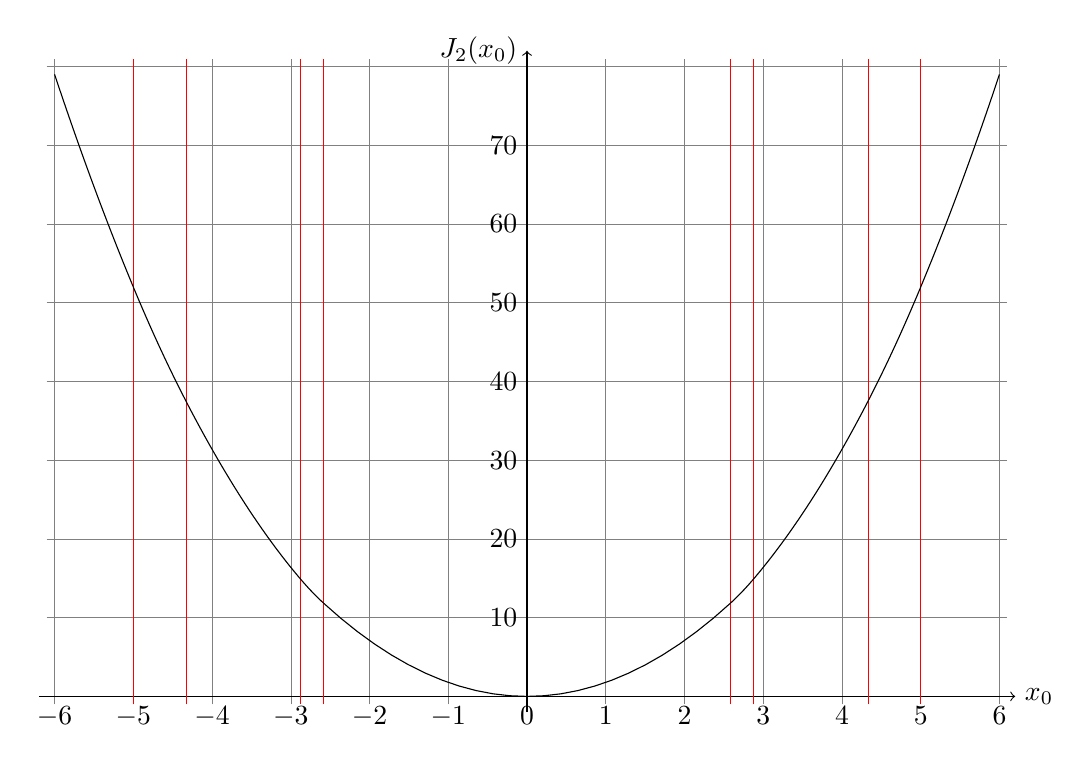
\begin{tikzpicture}
    \draw[very thin,color=gray] (-6.1,-0.1) grid (6.1,8.1);
    \foreach \x in {-6,-5,...,6} \draw (\x,0) node[below] {$\x$};
    \foreach \y in {10,20,...,70} \draw (0,\y/10) node[left] {$\y$};
    \draw[->] (-6.2,0) -- (6.2,0) node[right] {$x_0$};
    \draw[->] (0,-0.2) -- (0,8.2) node[left] {$J_2(x_0)$};
    \draw[very thin,red] (31/12,-.1) -- (31/12,8.1);
    \draw[very thin,red] (23/8,-.1) -- (23/8,8.1);
    \draw[very thin,red] (13/3,-.1) -- (13/3,8.1);
    \draw[very thin,red] (5,-.1) -- (5,8.1);
    \draw[very thin,red] (-31/12,-.1) -- (-31/12,8.1);
    \draw[very thin,red] (-23/8,-.1) -- (-23/8,8.1);
    \draw[very thin,red] (-13/3,-.1) -- (-13/3,8.1);
    \draw[very thin,red] (-5,-.1) -- (-5,8.1);
	% \draw (-31/12,1705/1440) plot[domain=-6:6] (\x,{55/310*pow(\x,2))}) (31/12,1705/1440);
    
 %    \draw (31/12,1705/1440) plot[domain=-6:6] (\x,{1/70*(124 - 96*\x + 31*pow( \x,2))}) (23/8,953/640);
	% \draw (-23/8,953/640) plot[domain=-6:6] (\x,{1/70*(124 + 96*\x + 31*pow( \x,2))}) (-31/12,1705/1440);

 %    \draw (23/8,953/640) plot[domain=-6:6] (\x,{1/50*(13 - 16*\x + 13*pow( \x,2))}) (13/3,338/90);
 %    \draw (-13/3,338/90) plot[domain=-6:6] (\x,{1/50*(13 + 16*\x + 13*pow( \x,2))}) (-23/8,953/640);

 %    \draw (13/3,338/90) plot[domain=-6:6] (\x,{1/20*(39 - 22*\x + 7*pow(\x,2))}) (5,52/10);
 %    \draw (-5,52/10) plot[domain=-6:6] (\x,{1/20*(39 + 22*\x + 7*pow(\x,2))}) (-13/3,338/90);

 %    \draw (5,52/10) plot[domain=-6:6] (\x,{(7 - 6*\x + 3*pow(\x,2))/10}) (6,79/10);
 %    \draw (-6,79/10) plot[domain=-6:6] (\x,{(7 + 6*\x + 3*pow(\x,2))/10}) (-5,52/10);

    \draw (-31/12,1705/1440) plot[domain=-31/12:31/12] (\x,{55/310*pow(\x,2))}) (31/12,1705/1440);
    
    \draw (31/12,1705/1440) plot[domain=2.58333:2.875] (\x,{1/70*(124 - 96*\x + 31*pow( \x,2))}) (23/8,953/640);
	\draw (-23/8,953/640) plot[domain=-2.875:-2.58333] (\x,{1/70*(124 + 96*\x + 31*pow( \x,2))}) (-31/12,1705/1440);

    \draw (23/8,953/640) plot[domain=2.875:4.33333] (\x,{1/50*(13 - 16*\x + 13*pow( \x,2))}) (13/3,338/90);
    \draw (-13/3,338/90) plot[domain=-4.33333:-2.875] (\x,{1/50*(13 + 16*\x + 13*pow( \x,2))}) (-23/8,953/640);

    \draw (13/3,338/90) plot[domain=4.33333:5] (\x,{1/20*(39 - 22*\x + 7*pow(\x,2))}) (5,52/10);
    \draw (-5,52/10) plot[domain=-5:-4.33333] (\x,{1/20*(39 + 22*\x + 7*pow(\x,2))}) (-13/3,338/90);

    \draw (5,52/10) plot[domain=5:6] (\x,{(7 - 6*\x + 3*pow(\x,2))/10}) (6,79/10);
    \draw (-6,79/10) plot[domain=-6:-5] (\x,{(7 + 6*\x + 3*pow(\x,2))/10}) (-5,52/10);
\end{tikzpicture}
\caption[Objective Value Function for One Dimensional Example]{Piecewise quadratic objective value of Example~\ref{example:linesearch} parametrised with respect to the initial state~$x_0$. In \textcolor{red}{red} we mark the boundaries of respective active sets.}
\label{figure:example:linesearch:objective}
\end{figure}
%
%
%
%
%
\begin{figure}\centering
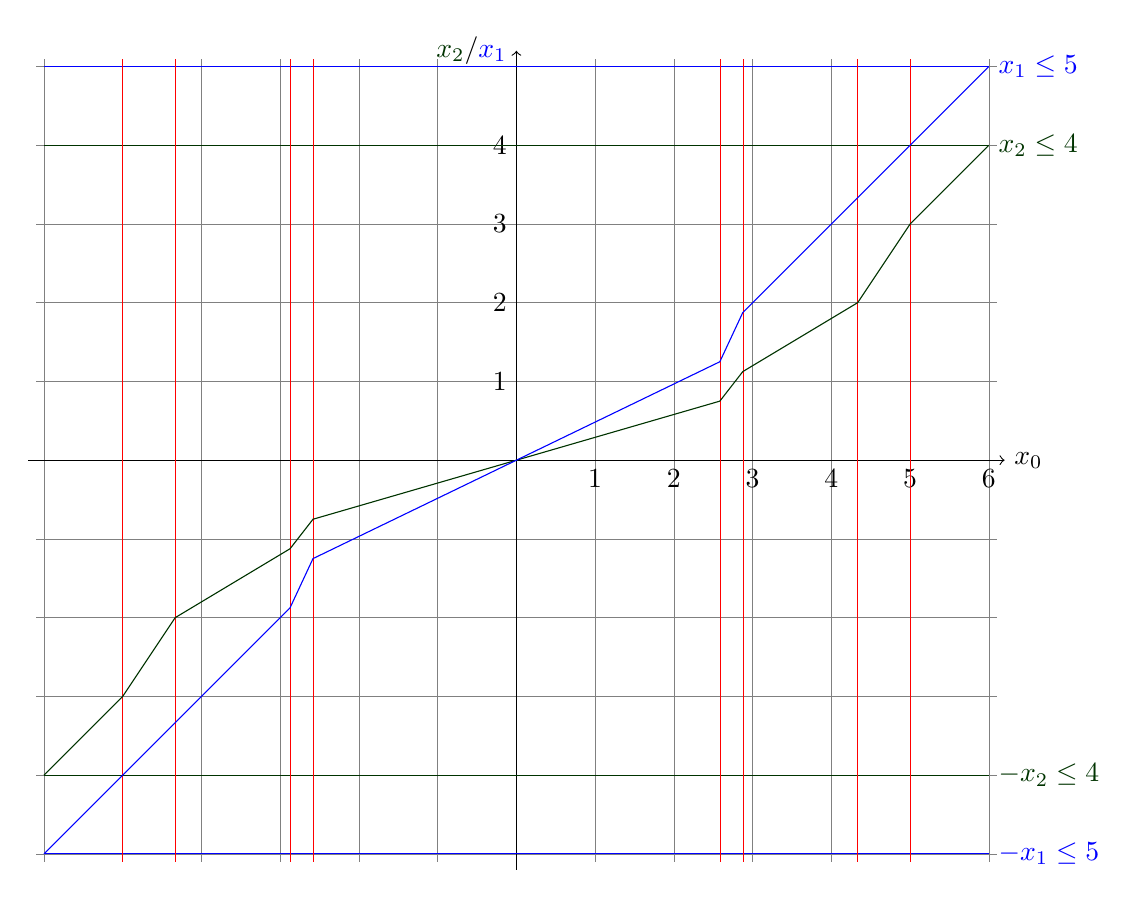
\begin{tikzpicture}
    \draw[very thin,color=gray] (-6.1,-5.1) grid (6.1,5.1);
    \foreach \x in {1,2,...,6} \draw (\x,0) node[below] {$\x$};
    \foreach \y in {1,2,...,4} \draw (0,\y) node[left] {$\y$};
    \draw[->] (-6.2,0) -- (6.2,0) node[right] {$x_0$};
    \draw[->] (0,-5.2) -- (0,5.2) node[left] {{\textcolor{black!80!green}{$x_2$}}/{\textcolor{blue}{$x_1$}}};
    \draw[black!80!green] (-6,4) -- (6,4) node[right] {$x_2\leq 4$};
    \draw[blue] (-6,5) -- (6,5) node[right] {$x_1\leq 5$};
    \draw[black!80!green] (-6,-4) -- (6,-4) node[right] {$-x_2\leq 4$};
    \draw[blue] (-6,-5) -- (6,-5) node[right] {$-x_1\leq 5$};
    \draw[very thin,red] (31/12,-5.1) -- (31/12,5.1);
    \draw[very thin,red] (23/8,-5.1) -- (23/8,5.1);
    \draw[very thin,red] (13/3,-5.1) -- (13/3,5.1);
    \draw[very thin,red] (5,-5.1) -- (5,5.1);
    \draw[very thin,red] (-31/12,-5.1) -- (-31/12,5.1);
    \draw[very thin,red] (-23/8,-5.1) -- (-23/8,5.1);
    \draw[very thin,red] (-13/3,-5.1) -- (-13/3,5.1);
    \draw[very thin,red] (-5,-5.1) -- (-5,5.1);
    \draw[black!80!green] (-6,-4) -- (-5,-3) -- (- 13/3,-2) -- (-23/8,-9/8) -- (-31/12,-3/4) -- (0,0) -- (31/12,3/4) -- (23/8,9/8) -- (13/3,2) -- (5,3) -- (6,4);
    \draw[blue] (-6,-5) -- (-5,-4) -- (-13/3,-10/3) -- (-23/8,-15/8) -- (-31/12,-5/4) -- (0,0) -- (31/12,5/4) -- (23/8,15/8) -- (13/3,10/3) -- (5,4) -- (6,5);
\end{tikzpicture}
\\[2em]
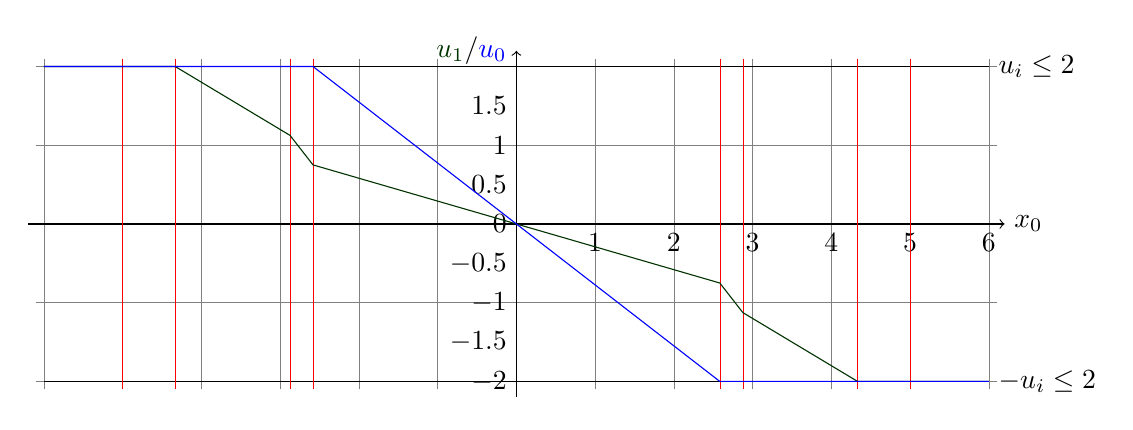
\begin{tikzpicture}
    \draw[very thin,color=gray] (-6.1,-2.1) grid (6.1,2.1);
    \foreach \x in {1,2,...,6} \draw (\x,0) node[below] {$\x$};
    \foreach \y in {-2,-1.5,...,1.5} \draw (0,\y) node[left] {$\y$};
    \draw[->] (-6.2,0) -- (6.2,0) node[right] {$x_0$};
    \draw[->] (0,-2.2) -- (0,2.2) node[left] {{\textcolor{black!80!green}{$u_1$}}/{\textcolor{blue}{$u_0$}}};
    \draw (-6,-2) -- (6,-2) node[right] {$-u_i\leq 2$};
    \draw (-6,2) -- (6,2) node[right] {$u_i\leq 2$};
    \draw[very thin,red] (31/12,2.1) -- (31/12,-2.1);
    \draw[very thin,red] (23/8,2.1) -- (23/8,-2.1);
    \draw[very thin,red] (13/3,2.1) -- (13/3,-2.1);
    \draw[very thin,red] (5,2.1) -- (5,-2.1);
    \draw[very thin,red] (-31/12,2.1) -- (-31/12,-2.1);
    \draw[very thin,red] (-23/8,2.1) -- (-23/8,-2.1);
    \draw[very thin,red] (-13/3,2.1) -- (-13/3,-2.1);
    \draw[very thin,red] (-5,2.1) -- (-5,-2.1);
    \draw[black!80!green] (-6,2) -- (-5,2) -- (-13/3,2) -- (-23/8,9/8) -- (-31/12,3/4) -- (0,0) -- (31/12,-3/4) -- (23/8,-9/8) -- (13/3,-2) -- (5,-2) -- (6,-2);
    \draw[blue] (-6,2) -- (-31/12,2) -- (0,0) -- (31/12,-2) -- (23/8,-2) -- (13/3,-2) -- (5,-2) -- (6,-2);
\end{tikzpicture}
\\[2em]
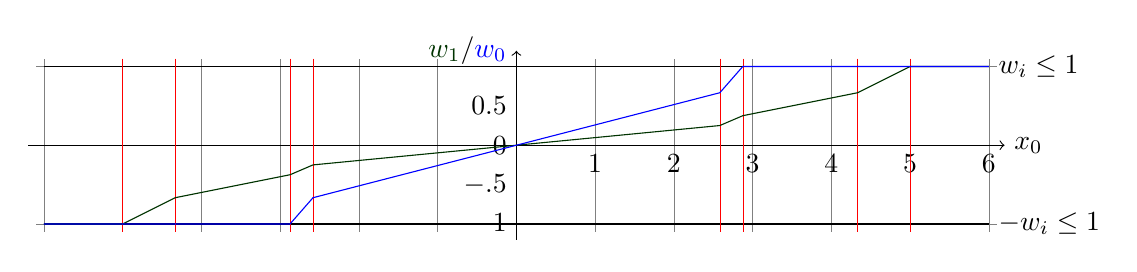
\begin{tikzpicture}
    \draw[very thin,color=gray] (-6.1,-1.1) grid (6.1,1.1);
    \foreach \x in {1,2,...,6} \draw (\x,0) node[below] {$\x$};
    \foreach \y in {-1,-.5,...,.5} \draw (0,\y) node[left] {$\y$};
    \draw[->] (-6.2,0) -- (6.2,0) node[right] {$x_0$};
    \draw[->] (0,-1.2) -- (0,1.2) node[left] {{\textcolor{black!80!green}{$w_1$}}/{\textcolor{blue}{$w_0$}}};
    \draw (-6,-1) -- (6,-1) node[right] {$-w_i\leq 1$};
    \draw (-6,1) -- (6,1) node[right] {$w_i\leq 1$};
    \draw[very thin,red] (31/12,1.1) -- (31/12,-1.1);
    \draw[very thin,red] (23/8,1.1) -- (23/8,-1.1);
    \draw[very thin,red] (13/3,1.1) -- (13/3,-1.1);
    \draw[very thin,red] (5,1.1) -- (5,-1.1);
    \draw[very thin,red] (-31/12,1.1) -- (-31/12,-1.1);
    \draw[very thin,red] (-23/8,1.1) -- (-23/8,-1.1);
    \draw[very thin,red] (-13/3,1.1) -- (-13/3,-1.1);
    \draw[very thin,red] (-5,1.1) -- (-5,-1.1);
    \draw[black!80!green] (-6,-1) -- (-5,-1) -- (-13/3,-2/3) -- (-23/8,-3/8) -- (-31/12,-1/4) -- (0,0) -- (31/12,1/4) -- (23/8,3/8) -- (13/3,2/3) -- (5,1) -- (6,1);
    \draw[blue] (-6,-1) -- (-23/8,-1)-- (-31/12,-2/3) -- (0,0) -- (31/12,2/3) -- (23/8,1) -- (13/3,1) -- (5,1) -- (6,1);
\end{tikzpicture}
\caption[Parametrised Solution to One Dimensional Example]{All decision variables for Example~\ref{example:linesearch} parametrised with respect to the initial state~$x_0$.}
\label{figure:example:linesearch:all:trajectories}
\end{figure}

\end{example}
%
%
\\[1em]
\mysplit We now discuss the approach to solving a general quadratic min-max sequence~\eqref{ch:quad:MPC:unspecific:constraints} using an active set solver, i.e. repeatedly solving equality constrained problems as discussed in section~\ref{ch:MPC:sec:qMPC:equality:constraints} and updating the set of active constraints as necessary.
%
\\[1em]
%
To summarise the notation used in the sequel we state the general Lagrangians of both subproblems at stage~$m$:
%
\begin{equation}\label{eq:lagrangian:equality:constraint:qmpc:problem}
	\begin{aligned}
	L_m &= \frac{1}{2} (x_k^TQx_k + u_k^TRu_k) + \hat J_m^\ast(x_k,u_k)+ \sum_{i\in\A_{\mathcal M_m}}\eta_{k,i}(E_{i,m}^x x_k- 1)\\&\quad + \xi_k^T(C_m^x x_k+ C_m^u u_k -\bfa{1})\\
	\hat L_m &= -\frac{\gamma^2}{2}w_k^Tw_k + J_{m-1}^\ast(x_{k+1}) + \sum_{i\in\A_{\W_m}}\zeta_{k,i}(G w_k - 1)\\&\quad + \hat\xi_k^T(\hat C_m x_k - \bfa{1}) + \lambda_{k}^T(x_{k+1}-Ax_k-Bu_k-w_k)
	\end{aligned}
\end{equation}
%
where~$k=N-m$ and $C_m,\hat C_m^{(\cdot)}$ denote the potential compatibility constraints.
%
In~\eqref{mpQP:solution} and~\eqref{mpQp:solution:second:stage} we derived the solution to equality constrained multi parametric quadratic min-max programs~\eqref{eq:lagrangian:equality:constraint:qmpc:problem}, which is affine with respect to its parameter.
%
By recursively substituting the parameters at stage~$m=i$ by the solution to at stage~$m=i+1$ we obtain an affine parametrisation of all decision variables with respect to the parameter at the initial stage~$m=N$, i.e. with respect to~$x_0$.
%
\begin{equation}\label{ch:mpc:qp:linesearch:all:decision:variables:parametrised}\begin{aligned}
	u_0(x_0) &= \Delta_{u_0}x_0 + \delta_{u_0} = V_{u_0}x_0 + v_{u_0}\\
	\eta_0(x_0,\hat\beta_0) &= \Sigma_{\eta_0,x_0}x_0 + \Sigma_{\eta_0,\hat\beta_0}\hat\beta_0+  \sigma_{\eta_0} = V_{\eta_0}x_0 + T_{\eta_0}\hat\beta_0 + v_{\eta_0}\\
	w_0(x_0) &= \Psi_{w_0}(x_0,u_0) + \psi_{w_0} = \Psi_{w_0}(I,V_{u_0})x_0 + \Psi v_{u_0} + \psi_{w_0} = V_{w_0}x_0+v_{w_0}\\
	&\quad\vdots\\
	\lambda_{N-1}(x_0,\hat\beta_0) &= \Upsilon_{\lambda_{N-1}}((V_{x_{N-1}},V_{u_{N-1}})x_0+(v_{x_{N-1}},v_{u_{N-1}}))\\
	&\quad\quad + \Upsilon_{\lambda_{N-1},\beta_{N-1}}(V_{\xi_{N-1}}x_0 + T_{\xi_{N-1}}\hat\beta_0+v_{\xi_{N-1}})+\upsilon_{\lambda_{N-1}}\\
	&= V_{\lambda_{N-1}}x_0+T_{\lambda_{N-1}}\hat\beta_0+v_{\lambda_{N-1}}
\end{aligned}\end{equation}
%
\begin{rem}
%
Recall that we choose the degeneracy parameters~$\beta_i,\hat\beta_i$ to be equal to the dual variable their compatibility constraint introduces, i.e. if $\xi_i$ and $\hat\xi_i$ denote the dual variable to the compatibility constraint at stage $m=i$ for the minimisation and maximisation respectively, we fix~$\beta_i = \xi_i$ and $\hat\beta_i = \xi_{i-1}$.
%
It is clear that if at stage~$m=N$ a compatibility constraint is active in the minimisation there is the additional parameter~$\hat\beta_0$, which can be used for any purpose.
%
It is therefore clear that~$T_{\cdot}$, which only affects dual variables, is only non-trivial when the minimisation at the initial stage~$m=N$ is degenerate.
%
\end{rem}
%
\noindent\mysplit For now assume that the minimisation at the initial stage~$m=N$ is not degenerate, i.e. all primal and dual variables are completely parametrised with respect to the initial state~$x_0$.
%
Due to their affine character all decision variables~\eqref{ch:mpc:qp:linesearch:all:decision:variables:parametrised} vary along a line in their respective spaces when the initial parameter varies along a line, i.e. $x_0(t) = \mathfrak{x}_0+t(\mathfrak{x}_e-\mathfrak{x}_0)$ implies $u_i(x_0(t)) = V_{u_i}(\mathfrak{x}_0+t(\mathfrak{x}_e-\mathfrak{x}_0)+v_{u_i} = V_{u_i}(\mathfrak{x}_e-\mathfrak{x}_0)t + (v_{u_i}+V_{u_i}\mathfrak{x}_0)$ and the same is true for all other variables.
%
Each primal variable is constrained by linear inequalities, that is all feasible solutions have to satisfy
%
\begin{subequations}\label{eq:linesearch:conditions}
\begin{equation}\label{eq:linesearch:conditions:primal}
	\begin{aligned}
	E_{i,m} (V_{x_k}(\mathfrak{x}_e-\mathfrak{x}_0)t + (v_{x_k}+V_{x_k}\mathfrak{x}_0)) \leq 1 \forall i\in M_{\X_m}, k\in\{0,\dots,N\}\\
	F_i (V_{u_k}(\mathfrak{x}_e-\mathfrak{x}_0)t + (v_{u_k}+V_{u_k}\mathfrak{x}_0))\leq 1 \forall i\in M_\U, k\in\{0,\dots,N-1\}\\
	G_i (V_{w_k}(\mathfrak{x}_e-\mathfrak{x}_0)t + (v_{w_k}+V_{w_k}\mathfrak{x}_0))\leq 1 \forall i\in M_\W, k\in\{0,\dots,N-1\}.\\
	\end{aligned}
\end{equation}
%
Also the dual variables~$\eta_k$ for $Fu_k\leq\bfa{1}$, $\zeta_k$ for $Gw_k\leq\bfa{1}$ and $\kappa_k$ for $E_mx_k\leq\bfa{1}$ have to satisfy
%
\begin{equation}\label{eq:linesearch:conditions:dual}\begin{aligned}
	V_{\eta_k}(\mathfrak{x}_e-\mathfrak{x}_0)t + (v_{\eta_k}+V_{\eta_k}\mathfrak{x}_0)\geq0\\
	V_{\zeta_k}(\mathfrak{x}_e-\mathfrak{x}_0)t + (v_{\zeta_k}+V_{u_k}\mathfrak{x}_0)\leq0\\
	V_{\kappa_k}(\mathfrak{x}_e-\mathfrak{x}_0)t + (v_{\kappa_k}+V_{u_k}\mathfrak{x}_0)\leq0
\end{aligned}\end{equation}
\end{subequations}
%
for all $k\in\{0,\dots,N-1\}$.
%
In order to determine the next active set of constraints we advance on the line~$x_0(t)$ with the maximal step without violating~\eqref{eq:linesearch:conditions}.
%
That is we solve the scalar linear program
%
\begin{equation}\label{eq:the:linesearch:lp}
	\begin{aligned}\max_t&\quad t\\
	\text{s.t.}&\quad \eqref{eq:linesearch:conditions}.
	\end{aligned}
\end{equation}
%
For any generic problem the solution $t^\ast$ to~\eqref{eq:the:linesearch:lp} is supported by exactly one inequality, i.e. no more than one inequality becomes active at each update of the active constraints.
%
If~$t^\ast$ is such that~$x_0(t^\ast)$ activates one of the primal constrains~\eqref{eq:linesearch:conditions:primal} we introduce that constraint as an active equality constraint and solve the updated problem.
%
Conversely, if~$t^\ast$ is such that~$x_0(t^\ast)$ activates one of the dual constraints~\eqref{eq:linesearch:conditions:dual} we remove the associated equality constraint and solve the updated problem.
%
Notice that in either case a change of the constraints at stage~$m=i$ has no effect on the solution of previous stages~$m<i$ and we can reduce the computational workload by only solving updated stages and reusing previous results.
%
\\[1em]
%
When the active set of constraints is updated in such a way that we have to introduce a compatibility constraint, then at that point its dual variable~$\xi_i$, $\hat\xi_i$ is zero and gains magnitude for increasing~$t$, it is effectively a ramp starting from~$t^\ast$.
%
Therefore the choice~$\beta_i = \hat\xi_i$, $\hat\beta_i = \xi_{i-1}$ guarantees continuous decision variables with respect to~$x_0$.
%
\\[1em]
%
\mysplit Now consider~$T_{\{\cdot\}}\neq0$, i.e. the constraints for the minimisation at stage~$m=N$ are linearly dependent.
%
Recall that for generic problems one constraint is added or removed at a time and therefore when the minimisation at stage~$m=N$ becomes degenerate there is exactly one linearly dependent constraint and the variable~$\hat\beta_0$ is a scalar.
%
In order to choose~$\hat\beta_0$ we use the dual problem to an equality constrained quadratic minimisation~\eqref{mpQP:second:stage}:
%
\begin{equation}\label{eq:non:trivial:beta:hat}\begin{aligned}
	\min_{u_0}&\quad \frac{1}{2}u_0^T(R+W_{N,u_0})u_0+c_{N,u_0}^Tu_0+d_N\\
	\text{s.t.}&\quad F_{\A_N}u_0 = \bfa{1}\\
	&\quad \hat C_N u_0 = \bfa{1}
\end{aligned}\end{equation}
%
with its Lagrangian
%
\begin{equation}
	\hat L_N = \frac{1}{2}u_0^T(R+W_{N,u_0})u_0+c_{N,u_0}^Tu_0+d_N + \eta_0^T(F_{\A_N}u_0-\bfa{1}) + \hat\xi_0^T(\hat C_N u_0-\bfa{1}),
\end{equation}
%
the dual problem is therefore given by
%
\begin{equation}\label{eq:dual:degenerate:problem:long:1}
	\begin{aligned}
	\max_{\eta_0,\hat\xi_0}&\quad - \frac{1}{2}\begin{pmatrix}\eta_0\\\hat\xi_0 \end{pmatrix}^T\begin{pmatrix}F_{\A_N}\\\hat C_N\end{pmatrix}^T(R+W_{N,u_0})^{-1}\begin{pmatrix}F_{\A_N}\\\hat C_N\end{pmatrix}\begin{pmatrix}\eta_0\\\hat\xi_0 \end{pmatrix}\\
	&\quad - \left(\begin{pmatrix}F_{\A_N}\\\hat C_N\end{pmatrix}-\begin{pmatrix}\bfa{1}\\\bfa{1}\end{pmatrix}\right)^T\begin{pmatrix}\eta_0\\\hat\xi_0 \end{pmatrix} +\frac{1}{2}c_{N,u_0}^T(R+W_{N,u_0})^{-1}c_{N,u_0} + d_N
	\end{aligned}
\end{equation}
%
where we abbreviate the primal and dual using $W_{N,u_0}$, $c_{N,u_0}$ are the terms corresponding to~$u_0$ in~$J_N(x_0,u_0)$, $d_N$ encapsulates the remaining parts which do not contain decision variables.
%
Using Lemma~\eqref{lem:mpQP:solution} the solution to~\eqref{eq:non:trivial:beta:hat} is given by
%
\begin{equation}
	\begin{aligned}
	u_0 &= \Delta_{u_0}x_0 + \delta_{u_0}\\
	\eta_0 &= \Sigma_{\eta_0,x_0} x_0 + \Sigma_{\eta_0,\hat\beta_0}\hat\beta_0 + \sigma_{\eta_0}\\
	\hat\xi_0 &= \Sigma_{\xi_0,x_0} x_0 + \Sigma_{\xi_0,\hat\beta_0}\hat\beta_0 + \sigma_{\xi_0}
	\end{aligned}
\end{equation}
%
with $F_{\A_N}^T\Sigma_{\eta_0,\hat\beta_0}+\hat C_N^T\Sigma_{\xi_0,\hat\beta_0}=0$.
%
With these identities the primal problem is already fixed by the value of~$x_0$, the dual on the other hand still has a degree of freedom.
%
In order to further advance with the line search we therefore use the constrained dual problem:
%
\begin{equation}
	\begin{aligned}
	\max_{\hat\beta_0}&\quad  (\bfa{1}^T\Sigma_{\eta_0,\hat\beta_0}+\bfa{1}\Sigma_{\xi_0,\hat\beta_0})\hat\beta_0\\
	\text{s.t.}&\quad T_{\eta_k}\hat\beta_0 + (V_{\eta_k}x_0+v_{\eta_k})\geq0\\
	&\quad T_{\zeta_k}\hat\beta_0 + (V_{\zeta_k}x_0+v_{\zeta_k})\leq0\\
	&\quad T_{\kappa_k}\hat\beta_0 + (V_{\kappa_k}x_0+v_{\kappa_k})\leq0\\
	&\quad k\in\{0,\dots,N-1\}
	\end{aligned}
\end{equation}
%
The active inequality constraint associated with the dual variable supporting the maximiser~$\hat\beta_0^\ast$ is then deactivated.
%
If the constraint to be deactivated is the last one that was activated the boundary of the feasible set is reached and~$\mathfrak{x}_e$ is infeasible, otherwise the line search continues without degeneracy.
%
We illustrate the entire algorithm involved in the line search in Figure~\ref{fig:flow:chart:line:search:standard}.
%
\begin{figure}
\centering
\begin{tikzpicture}[node distance=2cm]
\tikzstyle{startstop} = [rectangle, rounded corners=14, minimum width=3cm, minimum height=1cm,text centered, draw=black, fill=red!30]
\tikzstyle{io} = [trapezium, trapezium left angle=70, trapezium right angle=110, minimum width=3cm, minimum height=1cm, text centered, draw=black, fill=blue!30]
\tikzstyle{process} = [rectangle, minimum width=3cm, minimum height=1cm, text centered, draw=black, fill=orange!30]
\tikzstyle{decision} = [diamond, minimum width=3cm, minimum height=1cm, text centered, draw=black, fill=green!30]
\tikzstyle{arrow} = [thick,->,>=stealth]
\node (start) [startstop] {Initialisation};
\node (in1) [io, below of=start] {\begin{varwidth}{8em}Given $\mathfrak{x}_0$, $\A_m$, $\hat\A_{\hat m}$. Set $m^\ast=\hat m^\ast=1$\end{varwidth}};
\node (pro1) [process, below of=in1] {\begin{varwidth}{12em}Solve~$J_m^\ast(x_k)$ and $\hat J_{\hat m}^\ast(x,u)$ for $m\geq m^\ast$ and $\hat m\geq \hat m^\ast$.\end{varwidth}};
\node (dec1) [decision, below of=pro1, yshift=-0.5cm] {$T_{\{\cdot\}}=0$};
\node (decInfeasible) [decision, below left of=dec1,yshift=-.7cm] {2\textsuperscript{nd} time};
\node (inf) [startstop, left of=decInfeasible, xshift=-1.5cm] {Infeasible};
\node (dual) [process, below of=decInfeasible] {Solve~\eqref{eq:dual:degenerate:problem:long:1}};
\node (primal) [process, right of=decInfeasible,xshift=1.5cm] {Solve~\eqref{eq:the:linesearch:lp}};
\node (done) [decision, below of=primal] {$t\geq1$};
\node (finish) [startstop, right of=done,xshift=1.3cm] {Finish};
\node (morhatm) [decision, below left of=done,yshift=-.8cm,xshift=-.4cm] {$m^\ast$ or $\hat m^\ast$};
\node (hatm) [process, below left of=morhatm,yshift=-.8cm,xshift=-.4cm] {\begin{varwidth}{6em}Update~$\hat\A_{\hat m^\ast}$ set $m^\ast=\hat m^\ast$\end{varwidth}};
\node (mast) [process, below right of=morhatm,yshift=-.8cm,xshift=1.1cm] {\begin{varwidth}{10em}Update~$\A_{m^\ast}$ set~$\hat m^\ast=\min\{N,m^\ast+1\}$\end{varwidth}};
\node (help) [left of =inf,inner sep=-1,fill] {};
\node (help1) [right of=finish,inner sep=-1,fill] {};
\draw [arrow] (in1) -- (pro1);
\draw [arrow] (start) -- (in1);
\draw [arrow] (pro1) -- node[anchor=west,near end] {} (dec1);
\draw [arrow] (dec1) -- node[anchor=east,near start] {no} (decInfeasible);
\draw [arrow] (decInfeasible) --node[anchor=north] {yes} (inf);
\draw [arrow] (decInfeasible) --node[anchor=west] {no} (dual);
\draw [arrow] (dec1) --node[anchor=west] {yes} (primal);
\draw [arrow] (primal) -- (done);
\draw [arrow] (done) --node[above,near start] {yes} (finish);
\draw [arrow] (done) --node[anchor=west] {no} (morhatm);
\draw [arrow] (dual) -- (morhatm);
\draw [arrow] (morhatm) --node[anchor=east] {$\hat m^\ast$} (hatm);
\draw [arrow] (morhatm) --node[anchor=west] {$m^\ast$} (mast);
\draw [thick] (hatm) -| (help);
\draw [arrow] (help) |- (pro1);
\draw [thick] (mast) -| (help1);
\draw [arrow] (help1) |- (pro1);
\end{tikzpicture}
\caption[Flow chart illustrating line search]{Flow chart of the proposed line search. Here $\A_{m}$ and $\hat\A_{\hat m}$ denote the active constraints at sub-stage $m$ and $\hat m$ respectively, i.e. the $\hat\cdot$ variables relate to the sub-maximisation.
%
The \emph{2\textsuperscript{nd} time} conditional checks whether the $T_{\{\cdot\}}\neq0$ for two consecutive times.}
\label{fig:flow:chart:line:search:standard}
\end{figure}
%
\\[1em]
%
\mysplit A particular problem with active set solvers is that the number of active set changes between any two points can not easily be estimated.
%
We will now discuss why a realistic upper bound is unlikely to be found, for this we reformulate the described line-search in a more abstract form and relate it to the well understood simplex algorithm.
%
It is well known that the solution to a quadratic min-max program with linear constraints is a piecwise-quadratic function with respect to the parameter, see e.g.~\cite{Sun:1992,Tondel:2003,Baotic:2002}.
%
In particular the parameter space is decomposed into a polytopic complex~$\C$ such that for every convex polytope~$\mathcal P_i\in\C$ the solution to~\eqref{ch:quad:MPC:unspecific:constraints} is given by a quadratic function, i.e. $J_N(x) = \frac{1}{2}x^TQ_{\mathcal P_i}x +c_{\mathcal P_i}^Tx + d_{\mathcal P_i}$ for all $x\in\mathcal P_i$.
%
We can understand the line search to be an itinerary from $\mathfrak{x}_0\in\mathcal P_0$ to $\mathfrak{x}_e\in\mathcal P_e$, each update of the active set~$\mathcal A$ is directly related to the explicit objective value in the respective~$\mathcal P_i$.
%
Since the polytopic complex~$\mathcal C$ such that $x\in\abs{C}$ admits a feasible solition is bounded we first construct a polyhedral completion: For any bounded polytopic complex $\mathcal C=\bigcup_i\mathcal P_i\subset\RR^d$ we can find a finite number of polyhedra~$\mathcal O_j$ such that $\bigcup_i\mathcal P_i\cup\bigcup_j\mathcal O_j=\RR^d$.
%
We refer to $\bar{\mathcal C}:=\mathcal C\bigcup_j\mathcal O_j$ as the \emph{completed complex}, for the completed complex~$\bar{\mathcal C}$ we have the following definition.
%
\begin{defi}\label{def:complex:induced:polar:graph}
Let~$\bar{\mathcal C}$ be a completed complex, then its \emph{induced polar graph}~$\mathcal G^P(\bar{\mathcal C})=(\mathcal V,\mathcal E)$ is such that each element of~$\mathcal P_i\in\bar{\mathcal C}$ with full dimension~$\text{dim}(\mathcal P_i)=d$ corresponds to one vertex~$\nu_i\in\mathcal V$.
%
The edge set~$\mathcal E$ consists of pairs~$(\nu_i,\nu_j)$ for which corresponding, full dimensional elements of~$\mathcal P_i,\mathcal P_j\in\bar{\mathcal C}$ exist such that their intersection has a non-trivial relative interior~$\text{rel int}(\mathcal P_i\cap\mathcal P_j)\neq\emptyset$.
\end{defi}
%
\noindent Notice that here we define the \emph{polar} of the induced graph, this is because the induced graph (with vertex set directly corresponding to the vertices of the complex) is of little use in this discussion.
%
The condition on the relative interior can be understood as two full dimensional elements~$\mathcal P_i,\mathcal P_j\in\bar\C$ such that they share a face of dimension~$2$ or higher (sharing a vertex does not define a neighbourhood).
%
Since the completion we describe yields a polyhedral division of the space~$\RR^d$ it follows that the induced polar graph is $d$-connected.
%
The definition of the induced polar graph is illustrated in Figure~\ref{fig:graph:of:complex}.
%
\\[1em]
%
\mysplit By Definition~\ref{def:complex:induced:polar:graph} the induced polar graph of the polyhedral complex~$\bar{\mathcal C}$ is undirected, however we can define a canonical directed graph such that the direction is given by all paths connecting~$\nu_0$ and~$\nu_e$ without cycles, corresponding to a $d$-dimensional curve connecting~$\mathfrak{x}_0$ with~$\mathfrak{x}_e$ without intersecting itself.
%
Clearly, the itinerary of $x_0(t) = \mathfrak{x}_0+t(\mathfrak{x}_e-\mathfrak{x}_0)$ corresponds to one such path~$(\nu_0,\dots,\nu_e)$.
%
Recall the Hirsch conjuncture discussed in Section~\ref{ch:concepts:sec:polytopes}, which applies to $d$-connected graphs that arise from $d$-dimensional polytopes supported by $n$-hyperplanes and gives upper bounds on the diameter of the induced graph of such a polytope.
%
The reason the Hirsch conjuncture is so conservative is because the bound has to be constructed in two stages:
%
First the number of possible vertices has to be bounded for arbitrary polytopes in $\RR^d$ with $n$ inequalities and secondly those graphs have to be estimated for all possible configurations.
%
In the case of the line-search the situation is even more difficult, for the first step of the Hirsch conjuncture the number of vertices is bounded by the number of possible intersections of exactly $d$ hyperplanes (since $d$ hyperplanes support a vertex), the elements~$\mathcal P_i\in\bar{\mathcal C}$ on the other hand are given as intersections of half-spaces.
%
If the unconstrained solution of the min-max program is feasible anywhere, i.e. there exists a~$\mathcal P_i\in\bar{\mathcal C}$ such that for all $x\in\mathcal P_i$ the unconstrained solution applies, then $\mathcal P_i$ is given by the intersection of~$n$ half-spaces, for generic problems adjacent polytopes~$\mathcal P_j$ with $\text{rel int}(\mathcal P_i\cap\mathcal P_j)\neq\emptyset$ accordingly are given as an intersection of~$n-1$ half-spaces and so on up to~$n-d+1$.
%
The second stage of the Hirsch conjuncture bound would apply to the number of vertices obtained, however that number cannot be easily found and can only be upper bounded binomially which is over conservative for generic problems.
%
%
\\[1em]
%
\mysplit Due to the lack of a realistic upper bound on the number of active set changes, a study of the complexity of the proposed algorithm yields poor upper bounds.
%
However, the computational complexity of each min-max sequence can easily be bounded.
%
Notice that in the worst case scenario no more than~$2N$ multi parametric quadratic programs with equality constraints have to be solved.
%
Each multi parametric quadratic program with equality constraints is solved using Lemma~\ref{lem:mpQP:solution}, for this we have to compute one QR decomposition which requires no more than~$2(mn^2-\frac{n^3}{3})$ flops, where $m$ denotes the number of equality constraints and $n$ the number of decision variables, see~\cite{Golub:1996} for the particular flop counts.
%
Furthermore we require to invert a triangular matrix which costs no more than~$\frac{m^3-m}{6}$ flops and various matrix multiplication, each with $mnp$ flops (for $AB\in\RR^{m\times p}$ with $A\in\RR^{m\times n}, B\in\RR^{n\times p}$).
%
Potentially, the degenerate case in Lemma~\ref{lem:mpQP:solution} requires a Cholesky decomposition with no more than $\frac{n^3}{3}$ flops, to construct the solution we have to add up matrices, each addition adding another~$mn$ flops.
%
The worst case solution of Lemma~\ref{lem:mpQP:solution} can be shown to require no more than~$11n^3+n^2-\frac{n}{3}$ flops, this is done by using the proof of Lemma~\ref{lem:mpQP:solution} to determine an inverse (or pseudo inverse) solving the first order optimality conditions of the respective problem.
%
The solution is then constructed by multiplying the obtained (pseudo-)inverse with the constant and parameter dependent right hand side to obtain the solution, with this the optimal objective is evaluated to proceed with the next sub-problem.
%
Adding all these steps together we have that the maximal flop count required to solve the min-max recursion for any active set is no larger than $N(2d+5d^2+101d^3+8d^2(d+q_\U))$.
%
This means that the complexity of each min-max recursion depends linearly on the horizon.
%
Since a flop count might not be insightful we illustrate the time required to solve a two dimensional robust model predictive control problem of varying horizon length in Figure~\ref{fig:compelxity:of:linesearch}, where it can be seen that the slowest solution of an equality constraint min-max sequence~\textcolor{red}{$t_{\max}$} rises linearly in $N$ as predicted by its flop count.\footnote{%
The time measurements were acquired by simulation run in Matlab R2016a on a MacBook Pro 2012 clocked at 2.3 GHz.}
%
However, in this case the time required to solve the entire robust model predictive controller~\textcolor{blue}{$T_{total}$} seems to also rise linearly with the horizon length.
%
In previous publications we saw a quadratic correlation between~\textcolor{blue}{$T_{total}$} and $N$, see~\cite{Schaich:2015:ifac}, as mentioned before the relationship between the complexity of the line search and the horizon length is example dependent and not known in general.
%
\begin{figure}\centering
\begin{tikzpicture}
\draw[-latex'] (-.1,0) -- (10.2,0) node[below right] {$N$};
\draw[-latex',blue] (-.1,0) -- (-.1,4.2) node[above left] {$T_{total}$};
\draw[-latex',red] (0.1,0) -- (.1,4.2) node[above right] {$t_{\max}$};
\foreach \N in {1,2,...,50} \draw (\N/5,.02) -- (\N/5,-.02);
\foreach \N in {10,20,...,50} \draw (\N/5,-.02) node [below] {$\N$};
\foreach \t in {1,2,...,4} \draw[blue] (-.08,\t) -- (-.12,\t) node[left] {$\frac{\t}{16}$};
\foreach \T in {1,2,...,4} \draw[red] (.08,\T) -- (.12,\T) node[right] {$\frac{\T}{80}$};

\draw[red] (  0.2000,   0.8323) -- (  0.4000,   0.2248) -- (  0.6000,   0.1805) -- (  0.8000,   0.2221) -- (  1.0000,   0.2151) -- (  1.2000,   0.2865) -- (  1.4000,   0.2771) -- (  1.6000,   0.3663) -- (  1.8000,   0.3054) -- (  2.0000,   0.3442) -- (  2.2000,   0.4285) -- (  2.4000,   0.4197) -- (  2.6000,   0.4196) -- (  2.8000,   0.5085) -- (  3.0000,   0.5287) -- (  3.2000,   0.5685) -- (  3.4000,   0.5797) -- (  3.6000,   0.6431) -- (  3.8000,   0.6122) -- (  4.0000,   0.6632) -- (  4.2000,   0.6940) -- (  4.4000,   0.7647) -- (  4.6000,   0.8477) -- (  4.8000,   0.8171) -- (  5.0000,   0.8936) -- (  5.2000,   0.9302) -- (  5.4000,   0.9684) -- (  5.6000,   0.9326) -- (  5.8000,   1.0346) -- (  6.0000,   1.0870) -- (  6.2000,   1.1418) -- (  6.4000,   1.1500) -- (  6.6000,   1.2247) -- (  6.8000,   1.2501) -- (  7.0000,   1.2338) -- (  7.2000,   1.2912) -- (  7.4000,   1.3427) -- (  7.6000,   1.4848) -- (  7.8000,   1.4466) -- (  8.0000,   1.5805) -- (  8.2000,   1.5537) -- (  8.4000,   1.6487) -- (  8.6000,   1.6750) -- (  8.8000,   1.7138) -- (  9.0000,   1.7430) -- (  9.2000,   1.8649) -- (  9.4000,   2.7447) -- (  9.6000,   2.7590) -- (  9.8000,   2.8525) -- ( 10.0000,   3.0894);

\node at (  0.2000,   0.8323) [circle,red,scale=.2,draw] {};\node at (  0.4000,   0.2248) [circle,red,scale=.2,draw] {};\node at (  0.6000,   0.1805) [circle,red,scale=.2,draw] {};\node at (  0.8000,   0.2221) [circle,red,scale=.2,draw] {};\node at (  1.0000,   0.2151) [circle,red,scale=.2,draw] {};\node at (  1.2000,   0.2865) [circle,red,scale=.2,draw] {};\node at (  1.4000,   0.2771) [circle,red,scale=.2,draw] {};\node at (  1.6000,   0.3663) [circle,red,scale=.2,draw] {};\node at (  1.8000,   0.3054) [circle,red,scale=.2,draw] {};\node at (  2.0000,   0.3442) [circle,red,scale=.2,draw] {};\node at (  2.2000,   0.4285) [circle,red,scale=.2,draw] {};\node at (  2.4000,   0.4197) [circle,red,scale=.2,draw] {};\node at (  2.6000,   0.4196) [circle,red,scale=.2,draw] {};\node at (  2.8000,   0.5085) [circle,red,scale=.2,draw] {};\node at (  3.0000,   0.5287) [circle,red,scale=.2,draw] {};\node at (  3.2000,   0.5685) [circle,red,scale=.2,draw] {};\node at (  3.4000,   0.5797) [circle,red,scale=.2,draw] {};\node at (  3.6000,   0.6431) [circle,red,scale=.2,draw] {};\node at (  3.8000,   0.6122) [circle,red,scale=.2,draw] {};\node at (  4.0000,   0.6632) [circle,red,scale=.2,draw] {};\node at (  4.2000,   0.6940) [circle,red,scale=.2,draw] {};\node at (  4.4000,   0.7647) [circle,red,scale=.2,draw] {};\node at (  4.6000,   0.8477) [circle,red,scale=.2,draw] {};\node at (  4.8000,   0.8171) [circle,red,scale=.2,draw] {};\node at (  5.0000,   0.8936) [circle,red,scale=.2,draw] {};\node at (  5.2000,   0.9302) [circle,red,scale=.2,draw] {};\node at (  5.4000,   0.9684) [circle,red,scale=.2,draw] {};\node at (  5.6000,   0.9326) [circle,red,scale=.2,draw] {};\node at (  5.8000,   1.0346) [circle,red,scale=.2,draw] {};\node at (  6.0000,   1.0870) [circle,red,scale=.2,draw] {};\node at (  6.2000,   1.1418) [circle,red,scale=.2,draw] {};\node at (  6.4000,   1.1500) [circle,red,scale=.2,draw] {};\node at (  6.6000,   1.2247) [circle,red,scale=.2,draw] {};\node at (  6.8000,   1.2501) [circle,red,scale=.2,draw] {};\node at (  7.0000,   1.2338) [circle,red,scale=.2,draw] {};\node at (  7.2000,   1.2912) [circle,red,scale=.2,draw] {};\node at (  7.4000,   1.3427) [circle,red,scale=.2,draw] {};\node at (  7.6000,   1.4848) [circle,red,scale=.2,draw] {};\node at (  7.8000,   1.4466) [circle,red,scale=.2,draw] {};\node at (  8.0000,   1.5805) [circle,red,scale=.2,draw] {};\node at (  8.2000,   1.5537) [circle,red,scale=.2,draw] {};\node at (  8.4000,   1.6487) [circle,red,scale=.2,draw] {};\node at (  8.6000,   1.6750) [circle,red,scale=.2,draw] {};\node at (  8.8000,   1.7138) [circle,red,scale=.2,draw] {};\node at (  9.0000,   1.7430) [circle,red,scale=.2,draw] {};\node at (  9.2000,   1.8649) [circle,red,scale=.2,draw] {};\node at (  9.4000,   2.7447) [circle,red,scale=.2,draw] {};\node at (  9.6000,   2.7590) [circle,red,scale=.2,draw] {};\node at (  9.8000,   2.8525) [circle,red,scale=.2,draw] {};\node at ( 10.0000,   3.0894) [circle,red,scale=.2,draw] {};

\draw[blue] (  0.2000,   4.9675) -- (  0.4000,   2.6000) -- (  0.6000,   0.3891) -- (  0.8000,   0.3796) -- (  1.0000,   0.5966) -- (  1.2000,   0.4844) -- (  1.4000,   0.5621) -- (  1.6000,   0.3962) -- (  1.8000,   0.6406) -- (  2.0000,   0.5845) -- (  2.2000,   0.6807) -- (  2.4000,   0.8962) -- (  2.6000,   0.7479) -- (  2.8000,   0.7855) -- (  3.0000,   0.8255) -- (  3.2000,   0.8668) -- (  3.4000,   0.8968) -- (  3.6000,   0.9366) -- (  3.8000,   0.9934) -- (  4.0000,   0.9959) -- (  4.2000,   1.0534) -- (  4.4000,   1.0889) -- (  4.6000,   1.1235) -- (  4.8000,   1.1549) -- (  5.0000,   1.2024) -- (  5.2000,   1.3022) -- (  5.4000,   1.2997) -- (  5.6000,   1.6890) -- (  5.8000,   1.3283) -- (  6.0000,   1.4051) -- (  6.2000,   1.3836) -- (  6.4000,   1.5754) -- (  6.6000,   1.4713) -- (  6.8000,   1.5045) -- (  7.0000,   1.5646) -- (  7.2000,   1.5939) -- (  7.4000,   1.6280) -- (  7.6000,   1.6513) -- (  7.8000,   1.6854) -- (  8.0000,   1.7602) -- (  8.2000,   1.7056) -- (  8.4000,   1.6406) -- (  8.6000,   2.0583) -- (  8.8000,   1.7905) -- (  9.0000,   1.7601) -- (  9.2000,   2.0270) -- (  9.4000,   2.0944) -- (  9.6000,   2.0270) -- (  9.8000,   2.1640) -- ( 10.0000,   3.6372);

\node at (  0.2000,   4.9675) [rectangle,blue,scale=.2,draw] {};\node at (  0.4000,   2.6000) [rectangle,blue,scale=.2,draw] {};\node at (  0.6000,   0.3891) [rectangle,blue,scale=.2,draw] {};\node at (  0.8000,   0.3796) [rectangle,blue,scale=.2,draw] {};\node at (  1.0000,   0.5966) [rectangle,blue,scale=.2,draw] {};\node at (  1.2000,   0.4844) [rectangle,blue,scale=.2,draw] {};\node at (  1.4000,   0.5621) [rectangle,blue,scale=.2,draw] {};\node at (  1.6000,   0.3962) [rectangle,blue,scale=.2,draw] {};\node at (  1.8000,   0.6406) [rectangle,blue,scale=.2,draw] {};\node at (  2.0000,   0.5845) [rectangle,blue,scale=.2,draw] {};\node at (  2.2000,   0.6807) [rectangle,blue,scale=.2,draw] {};\node at (  2.4000,   0.8962) [rectangle,blue,scale=.2,draw] {};\node at (  2.6000,   0.7479) [rectangle,blue,scale=.2,draw] {};\node at (  2.8000,   0.7855) [rectangle,blue,scale=.2,draw] {};\node at (  3.0000,   0.8255) [rectangle,blue,scale=.2,draw] {};\node at (  3.2000,   0.8668) [rectangle,blue,scale=.2,draw] {};\node at (  3.4000,   0.8968) [rectangle,blue,scale=.2,draw] {};\node at (  3.6000,   0.9366) [rectangle,blue,scale=.2,draw] {};\node at (  3.8000,   0.9934) [rectangle,blue,scale=.2,draw] {};\node at (  4.0000,   0.9959) [rectangle,blue,scale=.2,draw] {};\node at (  4.2000,   1.0534) [rectangle,blue,scale=.2,draw] {};\node at (  4.4000,   1.0889) [rectangle,blue,scale=.2,draw] {};\node at (  4.6000,   1.1235) [rectangle,blue,scale=.2,draw] {};\node at (  4.8000,   1.1549) [rectangle,blue,scale=.2,draw] {};\node at (  5.0000,   1.2024) [rectangle,blue,scale=.2,draw] {};\node at (  5.2000,   1.3022) [rectangle,blue,scale=.2,draw] {};\node at (  5.4000,   1.2997) [rectangle,blue,scale=.2,draw] {};\node at (  5.6000,   1.6890) [rectangle,blue,scale=.2,draw] {};\node at (  5.8000,   1.3283) [rectangle,blue,scale=.2,draw] {};\node at (  6.0000,   1.4051) [rectangle,blue,scale=.2,draw] {};\node at (  6.2000,   1.3836) [rectangle,blue,scale=.2,draw] {};\node at (  6.4000,   1.5754) [rectangle,blue,scale=.2,draw] {};\node at (  6.6000,   1.4713) [rectangle,blue,scale=.2,draw] {};\node at (  6.8000,   1.5045) [rectangle,blue,scale=.2,draw] {};\node at (  7.0000,   1.5646) [rectangle,blue,scale=.2,draw] {};\node at (  7.2000,   1.5939) [rectangle,blue,scale=.2,draw] {};\node at (  7.4000,   1.6280) [rectangle,blue,scale=.2,draw] {};\node at (  7.6000,   1.6513) [rectangle,blue,scale=.2,draw] {};\node at (  7.8000,   1.6854) [rectangle,blue,scale=.2,draw] {};\node at (  8.0000,   1.7602) [rectangle,blue,scale=.2,draw] {};\node at (  8.2000,   1.7056) [rectangle,blue,scale=.2,draw] {};\node at (  8.4000,   1.6406) [rectangle,blue,scale=.2,draw] {};\node at (  8.6000,   2.0583) [rectangle,blue,scale=.2,draw] {};\node at (  8.8000,   1.7905) [rectangle,blue,scale=.2,draw] {};\node at (  9.0000,   1.7601) [rectangle,blue,scale=.2,draw] {};\node at (  9.2000,   2.0270) [rectangle,blue,scale=.2,draw] {};\node at (  9.4000,   2.0944) [rectangle,blue,scale=.2,draw] {};\node at (  9.6000,   2.0270) [rectangle,blue,scale=.2,draw] {};\node at (  9.8000,   2.1640) [rectangle,blue,scale=.2,draw] {};\node at ( 10.0000,   3.6372) [rectangle,blue,scale=.2,draw] {};
\end{tikzpicture}
\caption[Time cost of line search]{The time required to complete one line search from the origin~$\mathfrak{x}_0=0$ to the boundary of the respective feasible set~$\mathfrak{x}_e\in\partial\X_N$ for a two dimensional system.
%
The time \textcolor{red}{$t_{\max}$} is the maximal time required to solve one min-max recursion of length~$N$, whereas \textcolor{blue}{$T_{total}$} is the time required for the overall line search.
%
Both scales are in seconds.}
\label{fig:compelxity:of:linesearch}
\end{figure}
%
\begin{figure}\centering
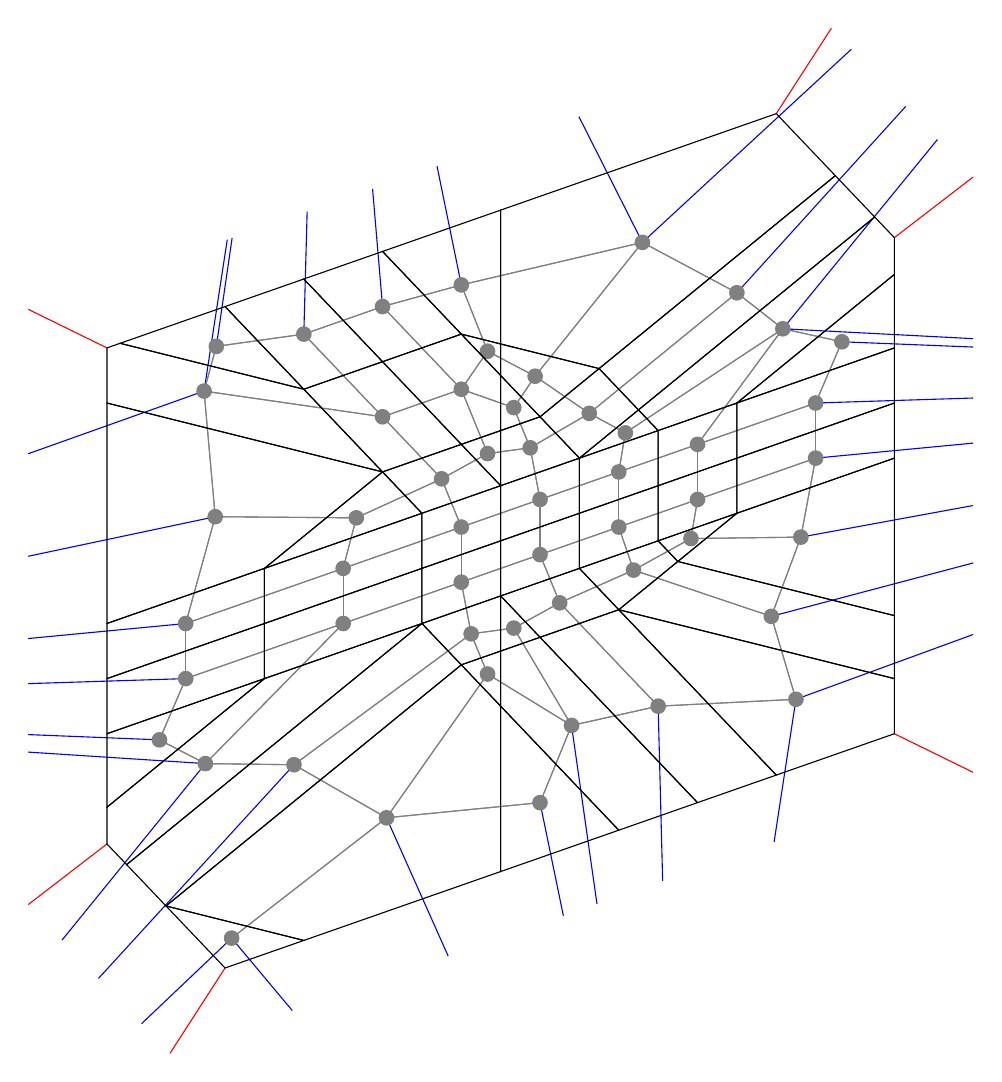
\begin{tikzpicture}[yscale=0.7]
\draw[blue] (  6.0000,   3.6679) -- (  3.5833,   3.8472);
\draw[blue] (  6.0000,   2.5909) -- (  4.0000,   2.5000);
\draw[blue] (  6.0000,   3.5156) -- (  4.3333,   3.6111);
\draw[blue] (  6.0000,   1.7727) -- (  4.0000,   1.5000);
\draw[blue] (  6.0000,  -0.4019) -- (  3.4375,  -1.3705);
\draw[blue] (  6.0000,  -1.7000) -- (  3.7500,  -2.8750);
\draw[blue] (  6.0000,   0.6405) -- (  3.8125,   0.0670);

\draw[blue] (  5.1450,   7.8825) -- (  3.0000,   4.5000);
\draw[blue] (  5.5466,   7.2800) -- (  3.5833,   3.8472);
\draw[blue] (  4.4539,   8.9191) -- (  1.8000,   5.4143);

\draw[blue] ( -3.4724,   5.4638) -- ( -3.7667,   2.7167);
\draw[blue] ( -2.4577,   5.9712) -- ( -2.5000,   3.7500);
\draw[blue] ( -1.6269,   6.3865) -- ( -1.5000,   4.2500);
\draw[blue] ( -3.4105,   5.4947) -- ( -3.6111,   3.5278);
\draw[blue] ( -0.8080,   6.7960) -- ( -0.5000,   4.6429);
\draw[blue] (  0.9934,   7.6967) -- (  1.8000,   5.4143);

\draw[blue] ( -6.0000,  -0.2802) -- ( -3.6250,   0.4375);
\draw[blue] ( -6.0000,   1.5801) -- ( -3.7667,   2.7167);
\draw[blue] ( -6.0000,  -1.7727) -- ( -4.0000,  -1.5000);
\draw[blue] ( -6.0000,  -2.5909) -- ( -4.0000,  -2.5000);
\draw[blue] ( -6.0000,  -3.8333) -- ( -3.7500,  -4.0417);
\draw[blue] ( -6.0000,  -3.5156) -- ( -4.3333,  -3.6111);

\draw[blue] ( -5.5705,  -7.2443) -- ( -3.7500,  -4.0417);
\draw[blue] ( -5.1073,  -7.9391) -- ( -2.6250,  -4.0625);
\draw[blue] ( -4.5600,  -8.7600) -- ( -3.4167,  -7.2083);

\draw[blue] (  2.0571,  -6.1714) -- (  2.0000,  -3.0000);
\draw[blue] (  1.2232,  -6.5884) -- (  0.9000,  -3.3500);
\draw[blue] ( -0.6668,  -7.5334) -- ( -1.4500,  -5.0250);
\draw[blue] (  3.4726,  -5.4637) -- (  3.7500,  -2.8750);
\draw[blue] (  0.7962,  -6.8019) -- (  0.5000,  -4.7500);
\draw[blue] ( -2.6460,  -8.5230) -- ( -3.4167,  -7.2083);


\draw[red] (  5.0000,  -3.5000) -- (  6.0000,  -4.2000);
\draw[red] (  5.0000,   5.5000) -- (  6.0000,   6.6000);
\draw[red] (  3.5000,   7.7500) -- (  4.2000,   9.3000);
\draw[red] ( -5.0000,   3.5000) -- ( -6.0000,   4.2000);
\draw[red] ( -5.0000,  -5.5000) -- ( -6.0000,  -6.6000);
\draw[red] ( -3.5000,  -7.7500) -- ( -4.2000,  -9.3000);


\node at ( -0.7500,   1.1250) [circle,fill=gray,scale=.6] {};
\draw[gray] ( -0.7500,   1.1250) -- ( -0.5000,   0.2500);
\draw[gray] ( -0.7500,   1.1250) -- ( -0.1667,   1.5833);
\draw[gray] ( -0.7500,   1.1250) -- ( -1.8333,   0.4167);
\draw[gray] ( -0.7500,   1.1250) -- ( -1.5000,   2.2500);
\node at ( -0.5000,   0.2500) [circle,fill=gray,scale=.6] {};
\draw[gray] ( -0.5000,   0.2500) -- ( -0.7500,   1.1250);
\draw[gray] ( -0.5000,   0.2500) -- (  0.5000,   0.7500);
\draw[gray] ( -0.5000,   0.2500) -- ( -2.0000,  -0.5000);
\draw[gray] ( -0.5000,   0.2500) -- ( -0.5000,  -0.7500);
\node at ( -0.1667,   1.5833) [circle,fill=gray,scale=.6] {};
\draw[gray] ( -0.1667,   1.5833) -- ( -0.7500,   1.1250);
\draw[gray] ( -0.1667,   1.5833) -- (  0.3750,   1.6875);
\draw[gray] ( -0.1667,   1.5833) -- ( -0.5000,   2.7500);
\node at ( -1.8333,   0.4167) [circle,fill=gray,scale=.6] {};
\draw[gray] ( -1.8333,   0.4167) -- ( -0.7500,   1.1250);
\draw[gray] ( -1.8333,   0.4167) -- ( -2.0000,  -0.5000);
\draw[gray] ( -1.8333,   0.4167) -- ( -3.6250,   0.4375);
\node at ( -1.5000,   2.2500) [circle,fill=gray,scale=.6] {};
\draw[gray] ( -1.5000,   2.2500) -- ( -0.7500,   1.1250);
\draw[gray] ( -1.5000,   2.2500) -- ( -0.5000,   2.7500);
\draw[gray] ( -1.5000,   2.2500) -- ( -3.7667,   2.7167);
\draw[gray] ( -1.5000,   2.2500) -- ( -2.5000,   3.7500);
\node at (  0.5000,   0.7500) [circle,fill=gray,scale=.6] {};
\draw[gray] (  0.5000,   0.7500) -- ( -0.5000,   0.2500);
\draw[gray] (  0.5000,   0.7500) -- (  0.3750,   1.6875);
\draw[gray] (  0.5000,   0.7500) -- (  1.5000,   1.2500);
\draw[gray] (  0.5000,   0.7500) -- (  0.5000,  -0.2500);
\node at ( -2.0000,  -0.5000) [circle,fill=gray,scale=.6] {};
\draw[gray] ( -2.0000,  -0.5000) -- ( -0.5000,   0.2500);
\draw[gray] ( -2.0000,  -0.5000) -- ( -1.8333,   0.4167);
\draw[gray] ( -2.0000,  -0.5000) -- ( -4.0000,  -1.5000);
\draw[gray] ( -2.0000,  -0.5000) -- ( -2.0000,  -1.5000);
\node at ( -0.5000,  -0.7500) [circle,fill=gray,scale=.6] {};
\draw[gray] ( -0.5000,  -0.7500) -- ( -0.5000,   0.2500);
\draw[gray] ( -0.5000,  -0.7500) -- (  0.5000,  -0.2500);
\draw[gray] ( -0.5000,  -0.7500) -- ( -2.0000,  -1.5000);
\draw[gray] ( -0.5000,  -0.7500) -- ( -0.3750,  -1.6875);
\node at (  0.3750,   1.6875) [circle,fill=gray,scale=.6] {};
\draw[gray] (  0.3750,   1.6875) -- ( -0.1667,   1.5833);
\draw[gray] (  0.3750,   1.6875) -- (  0.5000,   0.7500);
\draw[gray] (  0.3750,   1.6875) -- (  1.1250,   2.3125);
\draw[gray] (  0.3750,   1.6875) -- (  0.1667,   2.4167);
\node at ( -0.5000,   2.7500) [circle,fill=gray,scale=.6] {};
\draw[gray] ( -0.5000,   2.7500) -- ( -0.1667,   1.5833);
\draw[gray] ( -0.5000,   2.7500) -- ( -1.5000,   2.2500);
\draw[gray] ( -0.5000,   2.7500) -- (  0.1667,   2.4167);
\draw[gray] ( -0.5000,   2.7500) -- ( -0.1667,   3.4405);
\draw[gray] ( -0.5000,   2.7500) -- ( -1.5000,   4.2500);
\node at ( -3.6250,   0.4375) [circle,fill=gray,scale=.6] {};
\draw[gray] ( -3.6250,   0.4375) -- ( -1.8333,   0.4167);
\draw[gray] ( -3.6250,   0.4375) -- ( -3.7667,   2.7167);
\draw[gray] ( -3.6250,   0.4375) -- ( -4.0000,  -1.5000);
\node at ( -3.7667,   2.7167) [circle,fill=gray,scale=.6] {};
\draw[gray] ( -3.7667,   2.7167) -- ( -1.5000,   2.2500);
\draw[gray] ( -3.7667,   2.7167) -- ( -3.6250,   0.4375);
\draw[gray] ( -3.7667,   2.7167) -- ( -3.6111,   3.5278);
\node at ( -2.5000,   3.7500) [circle,fill=gray,scale=.6] {};
\draw[gray] ( -2.5000,   3.7500) -- ( -1.5000,   2.2500);
\draw[gray] ( -2.5000,   3.7500) -- ( -1.5000,   4.2500);
\draw[gray] ( -2.5000,   3.7500) -- ( -3.6111,   3.5278);
\node at (  1.5000,   1.2500) [circle,fill=gray,scale=.6] {};
\draw[gray] (  1.5000,   1.2500) -- (  0.5000,   0.7500);
\draw[gray] (  1.5000,   1.2500) -- (  1.5833,   1.9583);
\draw[gray] (  1.5000,   1.2500) -- (  2.5000,   1.7500);
\draw[gray] (  1.5000,   1.2500) -- (  1.5000,   0.2500);
\node at (  0.5000,  -0.2500) [circle,fill=gray,scale=.6] {};
\draw[gray] (  0.5000,  -0.2500) -- (  0.5000,   0.7500);
\draw[gray] (  0.5000,  -0.2500) -- ( -0.5000,  -0.7500);
\draw[gray] (  0.5000,  -0.2500) -- (  1.5000,   0.2500);
\draw[gray] (  0.5000,  -0.2500) -- (  0.7500,  -1.1250);
\node at ( -4.0000,  -1.5000) [circle,fill=gray,scale=.6] {};
\draw[gray] ( -4.0000,  -1.5000) -- ( -2.0000,  -0.5000);
\draw[gray] ( -4.0000,  -1.5000) -- ( -3.6250,   0.4375);
\draw[gray] ( -4.0000,  -1.5000) -- ( -4.0000,  -2.5000);
\node at ( -2.0000,  -1.5000) [circle,fill=gray,scale=.6] {};
\draw[gray] ( -2.0000,  -1.5000) -- ( -2.0000,  -0.5000);
\draw[gray] ( -2.0000,  -1.5000) -- ( -0.5000,  -0.7500);
\draw[gray] ( -2.0000,  -1.5000) -- ( -4.0000,  -2.5000);
\draw[gray] ( -2.0000,  -1.5000) -- ( -3.7500,  -4.0417);
\node at ( -0.3750,  -1.6875) [circle,fill=gray,scale=.6] {};
\draw[gray] ( -0.3750,  -1.6875) -- ( -0.5000,  -0.7500);
\draw[gray] ( -0.3750,  -1.6875) -- ( -0.1667,  -2.4167);
\draw[gray] ( -0.3750,  -1.6875) -- (  0.1667,  -1.5833);
\draw[gray] ( -0.3750,  -1.6875) -- ( -2.6250,  -4.0625);
\node at (  1.1250,   2.3125) [circle,fill=gray,scale=.6] {};
\draw[gray] (  1.1250,   2.3125) -- (  0.3750,   1.6875);
\draw[gray] (  1.1250,   2.3125) -- (  1.5833,   1.9583);
\draw[gray] (  1.1250,   2.3125) -- (  0.4375,   2.9866);
\draw[gray] (  1.1250,   2.3125) -- (  3.0000,   4.5000);
\node at (  0.1667,   2.4167) [circle,fill=gray,scale=.6] {};
\draw[gray] (  0.1667,   2.4167) -- (  0.3750,   1.6875);
\draw[gray] (  0.1667,   2.4167) -- ( -0.5000,   2.7500);
\draw[gray] (  0.1667,   2.4167) -- (  0.4375,   2.9866);
\node at ( -0.1667,   3.4405) [circle,fill=gray,scale=.6] {};
\draw[gray] ( -0.1667,   3.4405) -- ( -0.5000,   2.7500);
\draw[gray] ( -0.1667,   3.4405) -- (  0.4375,   2.9866);
\draw[gray] ( -0.1667,   3.4405) -- ( -0.5000,   4.6429);
\node at ( -1.5000,   4.2500) [circle,fill=gray,scale=.6] {};
\draw[gray] ( -1.5000,   4.2500) -- ( -0.5000,   2.7500);
\draw[gray] ( -1.5000,   4.2500) -- ( -2.5000,   3.7500);
\draw[gray] ( -1.5000,   4.2500) -- ( -0.5000,   4.6429);
\node at ( -3.6111,   3.5278) [circle,fill=gray,scale=.6] {};
\draw[gray] ( -3.6111,   3.5278) -- ( -3.7667,   2.7167);
\draw[gray] ( -3.6111,   3.5278) -- ( -2.5000,   3.7500);
\node at (  1.5833,   1.9583) [circle,fill=gray,scale=.6] {};
\draw[gray] (  1.5833,   1.9583) -- (  1.5000,   1.2500);
\draw[gray] (  1.5833,   1.9583) -- (  1.1250,   2.3125);
\draw[gray] (  1.5833,   1.9583) -- (  3.5833,   3.8472);
\node at (  2.5000,   1.7500) [circle,fill=gray,scale=.6] {};
\draw[gray] (  2.5000,   1.7500) -- (  1.5000,   1.2500);
\draw[gray] (  2.5000,   1.7500) -- (  3.5833,   3.8472);
\draw[gray] (  2.5000,   1.7500) -- (  4.0000,   2.5000);
\draw[gray] (  2.5000,   1.7500) -- (  2.5000,   0.7500);
\node at (  1.5000,   0.2500) [circle,fill=gray,scale=.6] {};
\draw[gray] (  1.5000,   0.2500) -- (  1.5000,   1.2500);
\draw[gray] (  1.5000,   0.2500) -- (  0.5000,  -0.2500);
\draw[gray] (  1.5000,   0.2500) -- (  2.5000,   0.7500);
\draw[gray] (  1.5000,   0.2500) -- (  1.6875,  -0.5312);
\node at (  0.7500,  -1.1250) [circle,fill=gray,scale=.6] {};
\draw[gray] (  0.7500,  -1.1250) -- (  0.5000,  -0.2500);
\draw[gray] (  0.7500,  -1.1250) -- (  0.1667,  -1.5833);
\draw[gray] (  0.7500,  -1.1250) -- (  1.6875,  -0.5312);
\draw[gray] (  0.7500,  -1.1250) -- (  2.0000,  -3.0000);
\node at ( -4.0000,  -2.5000) [circle,fill=gray,scale=.6] {};
\draw[gray] ( -4.0000,  -2.5000) -- ( -4.0000,  -1.5000);
\draw[gray] ( -4.0000,  -2.5000) -- ( -2.0000,  -1.5000);
\draw[gray] ( -4.0000,  -2.5000) -- ( -4.3333,  -3.6111);
\node at ( -3.7500,  -4.0417) [circle,fill=gray,scale=.6] {};
\draw[gray] ( -3.7500,  -4.0417) -- ( -2.0000,  -1.5000);
\draw[gray] ( -3.7500,  -4.0417) -- ( -2.6250,  -4.0625);
\draw[gray] ( -3.7500,  -4.0417) -- ( -4.3333,  -3.6111);
\node at ( -0.1667,  -2.4167) [circle,fill=gray,scale=.6] {};
\draw[gray] ( -0.1667,  -2.4167) -- ( -0.3750,  -1.6875);
\draw[gray] ( -0.1667,  -2.4167) -- (  0.9000,  -3.3500);
\draw[gray] ( -0.1667,  -2.4167) -- ( -1.4500,  -5.0250);
\node at (  0.1667,  -1.5833) [circle,fill=gray,scale=.6] {};
\draw[gray] (  0.1667,  -1.5833) -- ( -0.3750,  -1.6875);
\draw[gray] (  0.1667,  -1.5833) -- (  0.7500,  -1.1250);
\draw[gray] (  0.1667,  -1.5833) -- (  0.9000,  -3.3500);
\node at ( -2.6250,  -4.0625) [circle,fill=gray,scale=.6] {};
\draw[gray] ( -2.6250,  -4.0625) -- ( -0.3750,  -1.6875);
\draw[gray] ( -2.6250,  -4.0625) -- ( -3.7500,  -4.0417);
\draw[gray] ( -2.6250,  -4.0625) -- ( -1.4500,  -5.0250);
\node at (  0.4375,   2.9866) [circle,fill=gray,scale=.6] {};
\draw[gray] (  0.4375,   2.9866) -- (  1.1250,   2.3125);
\draw[gray] (  0.4375,   2.9866) -- (  0.1667,   2.4167);
\draw[gray] (  0.4375,   2.9866) -- ( -0.1667,   3.4405);
\draw[gray] (  0.4375,   2.9866) -- (  1.8000,   5.4143);
\node at (  3.0000,   4.5000) [circle,fill=gray,scale=.6] {};
\draw[gray] (  3.0000,   4.5000) -- (  1.1250,   2.3125);
\draw[gray] (  3.0000,   4.5000) -- (  3.5833,   3.8472);
\draw[gray] (  3.0000,   4.5000) -- (  1.8000,   5.4143);
\node at ( -0.5000,   4.6429) [circle,fill=gray,scale=.6] {};
\draw[gray] ( -0.5000,   4.6429) -- ( -0.1667,   3.4405);
\draw[gray] ( -0.5000,   4.6429) -- ( -1.5000,   4.2500);
\draw[gray] ( -0.5000,   4.6429) -- (  1.8000,   5.4143);
\node at (  3.5833,   3.8472) [circle,fill=gray,scale=.6] {};
\draw[gray] (  3.5833,   3.8472) -- (  1.5833,   1.9583);
\draw[gray] (  3.5833,   3.8472) -- (  2.5000,   1.7500);
\draw[gray] (  3.5833,   3.8472) -- (  3.0000,   4.5000);
\draw[gray] (  3.5833,   3.8472) -- (  4.3333,   3.6111);
\node at (  4.0000,   2.5000) [circle,fill=gray,scale=.6] {};
\draw[gray] (  4.0000,   2.5000) -- (  2.5000,   1.7500);
\draw[gray] (  4.0000,   2.5000) -- (  4.3333,   3.6111);
\draw[gray] (  4.0000,   2.5000) -- (  4.0000,   1.5000);
\node at (  2.5000,   0.7500) [circle,fill=gray,scale=.6] {};
\draw[gray] (  2.5000,   0.7500) -- (  2.5000,   1.7500);
\draw[gray] (  2.5000,   0.7500) -- (  1.5000,   0.2500);
\draw[gray] (  2.5000,   0.7500) -- (  4.0000,   1.5000);
\draw[gray] (  2.5000,   0.7500) -- (  2.4167,   0.0417);
\node at (  1.6875,  -0.5312) [circle,fill=gray,scale=.6] {};
\draw[gray] (  1.6875,  -0.5312) -- (  1.5000,   0.2500);
\draw[gray] (  1.6875,  -0.5312) -- (  0.7500,  -1.1250);
\draw[gray] (  1.6875,  -0.5312) -- (  2.4167,   0.0417);
\draw[gray] (  1.6875,  -0.5312) -- (  3.4375,  -1.3705);
\node at (  2.0000,  -3.0000) [circle,fill=gray,scale=.6] {};
\draw[gray] (  2.0000,  -3.0000) -- (  0.7500,  -1.1250);
\draw[gray] (  2.0000,  -3.0000) -- (  0.9000,  -3.3500);
\draw[gray] (  2.0000,  -3.0000) -- (  3.7500,  -2.8750);
\node at ( -4.3333,  -3.6111) [circle,fill=gray,scale=.6] {};
\draw[gray] ( -4.3333,  -3.6111) -- ( -4.0000,  -2.5000);
\draw[gray] ( -4.3333,  -3.6111) -- ( -3.7500,  -4.0417);
\node at (  0.9000,  -3.3500) [circle,fill=gray,scale=.6] {};
\draw[gray] (  0.9000,  -3.3500) -- ( -0.1667,  -2.4167);
\draw[gray] (  0.9000,  -3.3500) -- (  0.1667,  -1.5833);
\draw[gray] (  0.9000,  -3.3500) -- (  2.0000,  -3.0000);
\draw[gray] (  0.9000,  -3.3500) -- (  0.5000,  -4.7500);
\node at ( -1.4500,  -5.0250) [circle,fill=gray,scale=.6] {};
\draw[gray] ( -1.4500,  -5.0250) -- ( -0.1667,  -2.4167);
\draw[gray] ( -1.4500,  -5.0250) -- ( -2.6250,  -4.0625);
\draw[gray] ( -1.4500,  -5.0250) -- (  0.5000,  -4.7500);
\draw[gray] ( -1.4500,  -5.0250) -- ( -3.4167,  -7.2083);
\node at (  1.8000,   5.4143) [circle,fill=gray,scale=.6] {};
\draw[gray] (  1.8000,   5.4143) -- (  0.4375,   2.9866);
\draw[gray] (  1.8000,   5.4143) -- (  3.0000,   4.5000);
\draw[gray] (  1.8000,   5.4143) -- ( -0.5000,   4.6429);
\node at (  4.3333,   3.6111) [circle,fill=gray,scale=.6] {};
\draw[gray] (  4.3333,   3.6111) -- (  3.5833,   3.8472);
\draw[gray] (  4.3333,   3.6111) -- (  4.0000,   2.5000);
\node at (  4.0000,   1.5000) [circle,fill=gray,scale=.6] {};
\draw[gray] (  4.0000,   1.5000) -- (  4.0000,   2.5000);
\draw[gray] (  4.0000,   1.5000) -- (  2.5000,   0.7500);
\draw[gray] (  4.0000,   1.5000) -- (  3.8125,   0.0670);
\node at (  2.4167,   0.0417) [circle,fill=gray,scale=.6] {};
\draw[gray] (  2.4167,   0.0417) -- (  2.5000,   0.7500);
\draw[gray] (  2.4167,   0.0417) -- (  1.6875,  -0.5312);
\draw[gray] (  2.4167,   0.0417) -- (  3.8125,   0.0670);
\node at (  3.4375,  -1.3705) [circle,fill=gray,scale=.6] {};
\draw[gray] (  3.4375,  -1.3705) -- (  1.6875,  -0.5312);
\draw[gray] (  3.4375,  -1.3705) -- (  3.7500,  -2.8750);
\draw[gray] (  3.4375,  -1.3705) -- (  3.8125,   0.0670);
\node at (  3.7500,  -2.8750) [circle,fill=gray,scale=.6] {};
\draw[gray] (  3.7500,  -2.8750) -- (  2.0000,  -3.0000);
\draw[gray] (  3.7500,  -2.8750) -- (  3.4375,  -1.3705);
\node at (  0.5000,  -4.7500) [circle,fill=gray,scale=.6] {};
\draw[gray] (  0.5000,  -4.7500) -- (  0.9000,  -3.3500);
\draw[gray] (  0.5000,  -4.7500) -- ( -1.4500,  -5.0250);
\node at ( -3.4167,  -7.2083) [circle,fill=gray,scale=.6] {};
\draw[gray] ( -3.4167,  -7.2083) -- ( -1.4500,  -5.0250);
\node at (  3.8125,   0.0670) [circle,fill=gray,scale=.6] {};
\draw[gray] (  3.8125,   0.0670) -- (  4.0000,   1.5000);
\draw[gray] (  3.8125,   0.0670) -- (  2.4167,   0.0417);
\draw[gray] (  3.8125,   0.0670) -- (  3.4375,  -1.3705);



\draw ( -1.5000,   1.2500) -- ( -1.0000,   0.5000) -- (  0.0000,   1.0000) -- ( -0.5000,   1.7500) -- ( -1.5000,   1.2500) -- cycle;
\draw ( -1.0000,  -0.5000) -- (  0.0000,   0.0000) -- (  0.0000,   1.0000) -- ( -1.0000,   0.5000) -- ( -1.0000,  -0.5000) -- cycle;
\draw ( -0.5000,   1.7500) -- (  0.0000,   1.0000) -- (  0.0000,   2.0000) -- ( -0.5000,   1.7500) -- cycle;
\draw ( -1.5000,   1.2500) -- ( -3.0000,  -0.5000) -- ( -1.0000,   0.5000) -- ( -1.5000,   1.2500) -- cycle;
\draw ( -1.5000,   1.2500) -- ( -0.5000,   1.7500) -- ( -1.5000,   3.2500) -- ( -2.5000,   2.7500) -- ( -1.5000,   1.2500) -- cycle;
\draw (  0.0000,   0.0000) -- (  1.0000,   0.5000) -- (  1.0000,   1.5000) -- (  0.0000,   1.0000) -- (  0.0000,   0.0000) -- cycle;
\draw ( -3.0000,  -1.5000) -- ( -1.0000,  -0.5000) -- ( -1.0000,   0.5000) -- ( -3.0000,  -0.5000) -- ( -3.0000,  -1.5000) -- cycle;
\draw ( -1.0000,  -1.5000) -- (  0.0000,  -1.0000) -- (  0.0000,   0.0000) -- ( -1.0000,  -0.5000) -- ( -1.0000,  -1.5000) -- cycle;
\draw (  0.0000,   2.0000) -- (  0.0000,   1.0000) -- (  1.0000,   1.5000) -- (  0.5000,   2.2500) -- (  0.0000,   2.0000) -- cycle;
\draw ( -0.5000,   1.7500) -- (  0.0000,   2.0000) -- (  0.0000,   3.0000) -- ( -0.5000,   3.7500) -- ( -1.5000,   3.2500) -- ( -0.5000,   1.7500) -- cycle;
\draw ( -1.5000,   1.2500) -- ( -5.0000,   2.5000) -- ( -5.0000,  -1.5000) -- ( -3.0000,  -0.5000) -- ( -1.5000,   1.2500) -- cycle;
\draw ( -2.5000,   2.7500) -- ( -4.8333,   3.5833) -- ( -5.0000,   3.5000) -- ( -5.0000,   2.5000) -- ( -1.5000,   1.2500) -- ( -2.5000,   2.7500) -- cycle;
\draw ( -2.5000,   2.7500) -- ( -1.5000,   3.2500) -- ( -2.5000,   4.7500) -- ( -3.5000,   4.2500) -- ( -2.5000,   2.7500) -- cycle;
\draw (  1.0000,   0.5000) -- (  2.0000,   1.0000) -- (  2.0000,   2.0000) -- (  1.0000,   1.5000) -- (  1.0000,   0.5000) -- cycle;
\draw (  0.0000,  -1.0000) -- (  1.0000,  -0.5000) -- (  1.0000,   0.5000) -- (  0.0000,   0.0000) -- (  0.0000,  -1.0000) -- cycle;
\draw ( -3.0000,  -1.5000) -- ( -3.0000,  -0.5000) -- ( -5.0000,  -1.5000) -- ( -5.0000,  -2.5000) -- ( -3.0000,  -1.5000) -- cycle;
\draw ( -3.0000,  -2.5000) -- ( -1.0000,  -1.5000) -- ( -1.0000,  -0.5000) -- ( -3.0000,  -1.5000) -- ( -3.0000,  -2.5000) -- cycle;
\draw ( -1.0000,  -1.5000) -- ( -0.5000,  -2.2500) -- (  0.0000,  -2.0000) -- (  0.0000,  -1.0000) -- ( -1.0000,  -1.5000) -- cycle;
\draw (  1.2500,   3.1250) -- (  0.5000,   2.2500) -- (  1.0000,   1.5000) -- (  1.7500,   2.3750) -- (  1.2500,   3.1250) -- cycle;
\draw (  0.0000,   2.0000) -- (  0.5000,   2.2500) -- (  0.0000,   3.0000) -- (  0.0000,   2.0000) -- cycle;
\draw ( -0.5000,   3.7500) -- (  0.0000,   3.0000) -- (  0.0000,   3.5714) -- ( -0.5000,   3.7500) -- cycle;
\draw ( -1.5000,   3.2500) -- ( -0.5000,   3.7500) -- ( -1.5000,   5.2500) -- ( -2.5000,   4.7500) -- ( -1.5000,   3.2500) -- cycle;
\draw ( -2.5000,   2.7500) -- ( -3.5000,   4.2500) -- ( -4.8333,   3.5833) -- ( -2.5000,   2.7500) -- cycle;
\draw (  1.7500,   2.3750) -- (  1.0000,   1.5000) -- (  2.0000,   2.0000) -- (  1.7500,   2.3750) -- cycle;
\draw (  2.0000,   1.0000) -- (  3.0000,   1.5000) -- (  3.0000,   2.5000) -- (  2.0000,   2.0000) -- (  2.0000,   1.0000) -- cycle;
\draw (  1.0000,  -0.5000) -- (  2.0000,   0.0000) -- (  2.0000,   1.0000) -- (  1.0000,   0.5000) -- (  1.0000,  -0.5000) -- cycle;
\draw (  0.0000,  -1.0000) -- (  0.5000,  -1.7500) -- (  1.5000,  -1.2500) -- (  1.0000,  -0.5000) -- (  0.0000,  -1.0000) -- cycle;
\draw ( -3.0000,  -2.5000) -- ( -3.0000,  -1.5000) -- ( -5.0000,  -2.5000) -- ( -5.0000,  -3.5000) -- ( -3.0000,  -2.5000) -- cycle;
\draw ( -3.0000,  -2.5000) -- ( -5.0000,  -4.8333) -- ( -5.0000,  -5.5000) -- ( -4.7500,  -5.8750) -- ( -1.0000,  -1.5000) -- ( -3.0000,  -2.5000) -- cycle;
\draw ( -0.5000,  -2.2500) -- (  0.0000,  -3.0000) -- (  0.0000,  -2.0000) -- ( -0.5000,  -2.2500) -- cycle;
\draw (  0.0000,  -1.0000) -- (  0.0000,  -2.0000) -- (  0.5000,  -1.7500) -- (  0.0000,  -1.0000) -- cycle;
\draw ( -1.0000,  -1.5000) -- ( -4.7500,  -5.8750) -- ( -4.2500,  -6.6250) -- ( -0.5000,  -2.2500) -- ( -1.0000,  -1.5000) -- cycle;
\draw (  0.5000,   2.2500) -- (  1.2500,   3.1250) -- (  0.0000,   3.5714) -- (  0.0000,   3.0000) -- (  0.5000,   2.2500) -- cycle;
\draw (  1.2500,   3.1250) -- (  1.7500,   2.3750) -- (  4.7500,   5.8750) -- (  4.2500,   6.6250) -- (  1.2500,   3.1250) -- cycle;
\draw ( -0.5000,   3.7500) -- (  0.0000,   3.5714) -- (  0.0000,   6.0000) -- ( -1.5000,   5.2500) -- ( -0.5000,   3.7500) -- cycle;
\draw (  1.7500,   2.3750) -- (  2.0000,   2.0000) -- (  3.0000,   2.5000) -- (  5.0000,   4.8333) -- (  5.0000,   5.5000) -- (  4.7500,   5.8750) -- (  1.7500,   2.3750) -- cycle;
\draw (  3.0000,   1.5000) -- (  5.0000,   2.5000) -- (  5.0000,   3.5000) -- (  3.0000,   2.5000) -- (  3.0000,   1.5000) -- cycle;
\draw (  2.0000,   0.0000) -- (  3.0000,   0.5000) -- (  3.0000,   1.5000) -- (  2.0000,   1.0000) -- (  2.0000,   0.0000) -- cycle;
\draw (  2.0000,   0.0000) -- (  1.0000,  -0.5000) -- (  1.5000,  -1.2500) -- (  2.2500,  -0.3750) -- (  2.0000,   0.0000) -- cycle;
\draw (  0.5000,  -1.7500) -- (  2.5000,  -4.7500) -- (  3.5000,  -4.2500) -- (  1.5000,  -1.2500) -- (  0.5000,  -1.7500) -- cycle;
\draw ( -3.0000,  -2.5000) -- ( -5.0000,  -3.5000) -- ( -5.0000,  -4.8333) -- ( -3.0000,  -2.5000) -- cycle;
\draw (  0.0000,  -3.0000) -- (  1.5000,  -5.2500) -- (  2.5000,  -4.7500) -- (  0.5000,  -1.7500) -- (  0.0000,  -2.0000) -- (  0.0000,  -3.0000) -- cycle;
\draw ( -0.5000,  -2.2500) -- ( -4.2500,  -6.6250) -- ( -2.5000,  -7.2500) -- (  0.0000,  -6.0000) -- (  0.0000,  -3.0000) -- ( -0.5000,  -2.2500) -- cycle;
\draw (  1.2500,   3.1250) -- (  4.2500,   6.6250) -- (  3.5000,   7.7500) -- (  0.0000,   6.0000) -- (  0.0000,   3.5714) -- (  1.2500,   3.1250) -- cycle;
\draw (  3.0000,   2.5000) -- (  5.0000,   3.5000) -- (  5.0000,   4.8333) -- (  3.0000,   2.5000) -- cycle;
\draw (  3.0000,   0.5000) -- (  5.0000,   1.5000) -- (  5.0000,   2.5000) -- (  3.0000,   1.5000) -- (  3.0000,   0.5000) -- cycle;
\draw (  2.0000,   0.0000) -- (  2.2500,  -0.3750) -- (  3.0000,   0.5000) -- (  2.0000,   0.0000) -- cycle;
\draw (  5.0000,  -1.3571) -- (  2.2500,  -0.3750) -- (  1.5000,  -1.2500) -- (  5.0000,  -2.5000) -- (  5.0000,  -1.3571) -- cycle;
\draw (  1.5000,  -1.2500) -- (  3.5000,  -4.2500) -- (  5.0000,  -3.5000) -- (  5.0000,  -2.5000) -- (  1.5000,  -1.2500) -- cycle;
\draw (  0.0000,  -3.0000) -- (  0.0000,  -6.0000) -- (  1.5000,  -5.2500) -- (  0.0000,  -3.0000) -- cycle;
\draw ( -4.2500,  -6.6250) -- ( -3.5000,  -7.7500) -- ( -2.5000,  -7.2500) -- ( -4.2500,  -6.6250) -- cycle;
\draw (  2.2500,  -0.3750) -- (  5.0000,  -1.3571) -- (  5.0000,   1.5000) -- (  3.0000,   0.5000) -- (  2.2500,  -0.3750) -- cycle;
\end{tikzpicture}
\caption[Induced polar graph of a polytopic complex]{The polytopic complex~$\mathcal C=\bigcup_i\mathcal P_i$ in black, the polyhedral completion of the complex~$\mathcal O_i$ in \textcolor{red}{red}.
%
In \textcolor{gray}{grey} the induced graph of the complex, with the edges for the completion in \textcolor{blue}{blue}.
%
The completed graph is $2$-connected.}
\label{fig:graph:of:complex}
\end{figure}
%
%


\section{Stability}\label{ch:MPC:sec:qMPC:stability}
\resetforsection
%
%
%
%
%
In this section we discuss the stability properties of the closed-loop behaviour produced by using the the solution~$u=u_0(x)$ of the robust model predictive control problem~\eqref{ch:quad:MPC:unspecific:constraints}.
%
There are two conceptually different ways to study the stability of~\eqref{ch:quad:MPC:unspecific:constraints}, the first way is the functional way, i.e. leading to statement that the closed loop system maps bounded sequences to bounded sequences in a $H_\infty$ manner, see e.g~\cite{Mayne:2006}.
%
The second way is a geometrical way using the framework of input-to-state stability,  i.e. using a Lyapunov like function to characterise an invariant set for norm bound disturbances, see e.g.~\cite{Lazar:2008}.
%
\\[1em]
%
\mysplit First we present the $H_\infty$ result\footnote{
%
Again we follow the ideas presented in~\cite{Buerger:2016} adapted to our problem
}, recall the introduced the sub-problems
%
\[
\begin{aligned}
	\hat J_m^\ast(x,u) &= \max_w J_{m-1}^\ast(Ax+Bu+w)\\
	J_m^\ast(x) &= \min_u \hat J_m^\ast(x,u)
\end{aligned}
\]
%
where we omit repeating the remaining constraints which are in the respective optimisation programs.
%
Using $k = N-m$ we use the notation $\hat J_m^\ast(x,u) = J_{m-1}^\ast(Ax+Bu+w_{k}(x,u))$ and $J_m^\ast(x) = \hat J_m^\ast(x,u_k(x))$ for the respective optimisers.
%
Let~$x\in\X_{m-1}$, then $u_{k+1}(x)\in\U$ exists and due to optimality we have~$J_m^\ast(x) = \hat J_m^\ast(x,u_k(x))\leq \hat J_m^\ast(x,u_{k+1}(x))$, similarly $\X_m\subseteq\X_{m+1}$ implies that $w_{k-1}(x,u)$ is admissible in~$\hat J_m^\ast(x,u) = J_{m-1}^\ast(Ax+Bu+w_{k}(x,u))\geq\hat J_{m-1}^\ast(Ax+Bu+w_{k-1}(x,u))$.
%
Furthermore due to the way the set sequence~$\X_m$ is defined, we have that~$x\in\X_m$ implies $Ax+Bu_k(x)+w\in\X_{m-1}$ for all $w\in\W$.
%
We can recursively use this to obtain
%
\begin{equation}\begin{aligned}
	J_m^\ast(x)-J_{m-1}^\ast(x)&\leq\hat J_m^\ast(x,u_{k+1}(x))-\hat J_{m-1}^\ast(x,u_{k+1}(x))\\
	\hat J_m^\ast(x,u) - \hat J_{m-1}^\ast(x,u) &\leq J_{m-1}^\ast(Ax+Bu+w_k(x,u))-J_{m-2}^\ast(Ax+Bu+w_{k}(x,u))
\end{aligned}\end{equation}
%
which leads us to the penultimate stage~$m=1$ where for~$x\in\X_0=\X_{\max}^\infty$ we have:
%
\begin{equation}
	J_1^\ast(x) - J_0^\ast(x) = \min_u\max_w \frac{1}{2}\left(x^TQx+u^TRu-\gamma^2w^Tw\right) + J_0^\ast(Ax+Bu+w)- J_0(x)
\end{equation}
%
which implies that we can apply the terminal controller~$u=Kx$, but the terminal controller was designed to satisfy
%
\begin{equation}
	J_0^\ast(x)-J_0^\ast(Ax+BKx+w)\geq\frac{1}{2}\left(x^TQx+(Kx)^TRKx-\gamma^2w^Tw\right)
\end{equation}
%
for all $w\in\RR^d$.\footnote{See Appendix~\ref{app:terminal:controller} for the design.}
%
But this yields $J_1^\ast(x) - J_0^\ast(x)\leq0$ and hence~$J_m^\ast(x)-J_{m-1}^\ast(x)\leq 0$, i.e. with our choice of the terminal conditions applying a longer horizon controller is \emph{cheaper} than applying shorter horizon one.
%
For the closed-loop system with initial state~$\mathfrak{x}_0$ using the controller~$u=u_0(x)$ we have
%
\begin{equation}\label{eq:decrease:of:cost:function}\begin{aligned}
	J_N^\ast(\mathfrak{x}_0) &= \min_u\max_w \frac{1}{2}\left(\mathfrak{x}_0^TQ\mathfrak{x}_0+u^TRu-\gamma^2w^Tw\right) + J_{N-1}^\ast(A\mathfrak{x}_0+Bu+w)\\
	&\geq \frac{1}{2}\left(\mathfrak{x}_0^TQ\mathfrak{x}_0+u_0(\mathfrak{x}_0)^TRu_0(\mathfrak{x}_0)-\gamma^2\mathfrak{w}_0^T\mathfrak{w}_0\right) + J_{N-1}^\ast(\underbrace{A\mathfrak{x}_0+Bu_0(\mathfrak{x}_0)+\mathfrak{w}_0}_{\mathfrak{x}_1})\\
	&\geq \frac{1}{2}\left(\mathfrak{x}_0^TQ\mathfrak{x}_0+u_0(\mathfrak{x}_0)^TR u_0(\mathfrak{x}_0)-\gamma^2\mathfrak{w}_0^T\mathfrak{w}_0\right) + J_{N}^\ast(\mathfrak{x}_1)\\
	&\geq \sum_{l=0}^n \frac{1}{2}\left(\mathfrak{x}_l^TQ\mathfrak{x}_l+u_0(\mathfrak{x}_l)^TRu_0(\mathfrak{x}_l)-\gamma^2\mathfrak{w}_l^T\mathfrak{w}_l\right) + J_{N}^\ast(\mathfrak{x}_{n+1})
\end{aligned}\end{equation}
%
or equivalently
%
\begin{equation}\label{eq:upper:bound:using:gamma}
	\gamma^2 \sum_{l=0}^n \mathfrak{w}_l^T\mathfrak{w}_l \geq \sum_{l=0}^n \mathfrak{x}_l^TQ\mathfrak{x}_l+u_0(\mathfrak{x}_l)^TRu_0(\mathfrak{x}_l) + 2\left(J_N^\ast(\mathfrak{x}_{n+1})-J_N^\ast(\mathfrak{x}_0)\right)
\end{equation}
%
Assume $\mathfrak{w}\in\ell_2(\W)$, i.e. $\sum_{l=0}^\infty\mathfrak{w}_l^T\mathfrak{w}_l\leq\infty$ then the right hand side of~\eqref{eq:upper:bound:using:gamma} is finite. 
%
Since we assume $Q\succeq0$, $R\succ0$ and due to the piecewise affine character of~$k(x)$ there exist $S_l\succ0$ such that
%
\[
	\mathfrak{x}_l^TQ\mathfrak{x}_l+u_0(\mathfrak{x}_l)^TRu_0(\mathfrak{x}_l)\geq \mathfrak{x}_l^T S_l\mathfrak{x}_l
\]
%
and with $S:=\liminf_{l\geq0}S_l\succ0$ we have
%
\[
	\gamma^2 \sum_{l=0}^n \mathfrak{w}_l^T\mathfrak{w}_l \geq \sum_{l=0}^n \mathfrak{x}_l^TS\mathfrak{x}_l +\underbrace{2\left(J_N^\ast(\mathfrak{x}_{n+1})-J_N^\ast(\mathfrak{x}_0)\right)}_{c_n}.
\]
%
So that $\sum_{l=0}^n \mathfrak{x}_l^TS\mathfrak{x}_l\geq \underline{\sigma}(S)^2\sum_{l=0}^n \mathfrak{x}_l^T\mathfrak{x}_l$ with the smallest eigenvalue of $S$ denoted by~$\underline{\sigma}(S)$.
%
The value of $c_n$ may fluctuate, it is however bounded in magnitude, to see this we recall that~$\mathfrak{x}_0\in\X_N$ guarantees that~$\mathfrak{x}_1\in\X_{N-1}\subseteq\X_N$ due to the way the stage constraints~$\X_m$ are defined. 
%
We therefore know that $\norm{\mathfrak{x}_0-\mathfrak{x}_l}_2$ is bounded by the diameter of $\X_N$, i.e.~$\norm{\mathfrak{x}_0-\mathfrak{x}_l}_2\leq 2 d(\{0\},\X_N)$.
%
Furthermore, we have seen that $J_N^\ast(x)$ is a continuous piecewise quadratic function in~$x\in\X_N$ with a finite number of quadratic components, since~$\X_N$ is compact we can therefore find a global Lipschitz constant~$L$ such that $\abs{J_N^\ast(\mathfrak{x}_{n+1})-J_N^\ast(\mathfrak{x}_0)}\leq L\norm{\mathfrak{x}_0-\mathfrak{x}_{n+1}}_2\leq2L d(\{0\},\X_N)$.
%
Now we can define a meaningful limit to obtain
%
\begin{equation}
	\gamma^2 \sum_{l=0}^\infty \mathfrak{w}_l^T\mathfrak{w}_l \geq \underline{\sigma}(S)^2\sum_{l=0}^\infty \mathfrak{x}_l^T\mathfrak{x}_l + \Delta
\end{equation}
%
This means that the closed-loop system maps $\ell_2(\W)$ to $\ell_2(\X_N)$ with the gain no larger than~$\frac{\gamma}{\underline{\sigma}(S)}$
%
\begin{equation}\label{eq:ell2:bound:on:closed:loop:system}
	\sup_{\substack{w\in\ell_2(\W)\\ \norm{w}_2\neq0}} \frac{\norm{x}_2^2}{\norm{w}_2^2}\leq\frac{\gamma^2}{\underline{\sigma}(S)^2} + \frac{\Delta}{\underline{\sigma}(S)^2\norm{w}_2^2}
\end{equation}
%
The bound~\eqref{eq:ell2:bound:on:closed:loop:system} implies that $\gamma$ bounds the the $H_\infty$-norm of the closed loop system.
%
\\[1em]
%
\mysplit The input-to-state stability derivation uses a similar line of arguments.
%
First we give a definition of input-to-state stability 
%
\begin{defi} 
The system~$x^+=f(x,w)$ is called input-to-state stable (see~\cite{Jiang:2001}) if there exists a $\KL$ function~$\alpha$ and a $\mathscr K$ function~$\beta$ such that
%
\[
\norm{x_k}_2\leq\alpha(\norm{x_0}_2,k)+\beta(\norm{w}_\infty)
\]
%
holds.
\end{defi}
%
\noindent A more useful characterisation of the input-to-state stability is given by using an input-to-state stability Lyapunov function
%
\begin{defi}
A continuous function~$V:\RR^d\rightarrow\RR^d$ is called ISS Lyapunov function for the system~$x^+=f(x,w)$ if there exist~$\underline{\alpha},\bar\alpha,\beta~\in\mathscr K^\infty$ and $\delta\in\mathscr K$ such that
\begin{align}
\underline\alpha(\norm{x}_2)&\leq V(x)\leq \bar\alpha(\norm{x}_2)\\
V(f(x,w))&-V(x)\leq -\beta(\norm{x}_2)+\delta(\norm{w}_2)
\end{align}
holds for all~$x,w\in\RR^d$.
\end{defi}
%
\noindent It is a well-known result that if a system~$x^+=f(x,u)$ admits an ISS Lyapunov function it is input-to-state stable, see~\cite{Jiang:2001} for details.
%
\\[1em]
%
We will now demonstrate that the closed loop system~$x^+=Ax+Bu_0(x)+w =: f(x,w)$ is input-to-state stable by showing that the optimal value function~$J_N^\ast(x)=:V(x)$ is an ISS Lyapunov function:
%
\begin{enumerate}
\item First we show that there exists an~$\underline\alpha\in\mathscr K$ such that $\underline\alpha(\norm{x}_2)\leq V(x)$.
%
Notice that for $x_0=0$ we have $J_N^\ast(x_0)=0$ and is locally purely quadratic, this can be seen by recursively solving all unconstrained maximisations and minimisations recursively, all decision variables depend linearly on the initial state~$x_0$.
%
Since all stage costs are purely quadratic and the optimisers are linear in $x_0$ the cost~$J_N(x_0)$ is a sum of purely quadratic terms and hence itself purely quadratic.
%
Furthermore notice that throughout this work we assumed that each minimisation and maximisation admits a unique solution, i.e. $\max_{w,x^+}-\frac{\gamma^2}{2} w^Tw + J_{m-1}^\ast(x^+)$ is assumed to be a strictly concave problem (in the sense of Lemma~\ref{thm:convex:non-convex:qp}) and $\min_{u}\frac{1}{2} u^T R u +\hat J_{m}(x,u)$ a strictly convex one.
%
Recall that the conjunction of a strictly convex function and an affine function is strictly convex, $f(x)$ strictly convex implies that $f(Ax+b)$ is strictly convex.
%
And hence we have 
%
\begin{equation}
	J_N^\ast(x_0) = \frac{1}{2}x_0^T \underbrace{Q}_{\succeq0}x_0 + \underbrace{\frac{1}{2}u_0(x_0)^TR u_0(x_0) + \hat J_{N}(x_0,u_0(x_0))}_{(\ast)}
\end{equation}
%
with $(\ast)$ strictly convex in~$x_0$, so that $J_N^\ast(x)$ is strictly convex in~$x$, piecewise quadratic and has its unique minimum at $x=0$, since its domain~$\X_N$ is compact we can find a purely quadratic lower bound~$\alpha_1 x^Tx\leq J_N^\ast(x)$.
%
\item With the same line of argument we can find a quadratic bound $\alpha_2x^Tx\geq J_N^\ast(x)$, so that we have $\underline\alpha(t)=\alpha_1t^2$ and $\bar\alpha(t)=\alpha_2t^2$.
%
\item Now we show that $J_N^\ast(Ax+Bu_0(x)+w)-J_N^\ast(x)\leq-\beta(\norm{x}_2)+\delta(\norm{w}_2)$, in fact we showed this decrease in the objective already in~\eqref{eq:decrease:of:cost:function} where we showed
%
\begin{equation}\begin{aligned}
	J_N^\ast(f(x,w))-J_N^\ast(x)&\leq -\frac{1}{2}\left( xQx+u_0(x)^TRu_0(x)\right)+\frac{\gamma^2}{2}w^Tw\\
	&\leq -\frac{\underline\sigma(S)^2}{2}x^Tx + \frac{\gamma^2}{2}w^Tw
\end{aligned}\end{equation}
\end{enumerate}
%
So that we can summarise the result as
%
\begin{thm}\label{thm:stability:statement}
The uncertain closed loop system~$\Sigma:x^+=Ax+Bu_0(x)+w$ discussed above maps $\Sigma:\ell_2(\W)\rightarrow\ell_2(\X_n)$ with an $H_\infty$ gain~\eqref{eq:ell2:bound:on:closed:loop:system}.
%
\\[1em]
%
Furthermore, the objective cost~$J_N^\ast(x)$ is an ISS Lyapunov function for the system satisfying
%
\begin{equation}
	\begin{aligned}
	\alpha_1\norm{x}_2^2&\leq J_N^\ast(x)\leq\alpha_2\norm{x}_2^2\\
	J_N^\ast(Ax+Bu_0(x)+w)-J_N^\ast(x)&\leq -\frac{\left(\underline\sigma(S)\norm{x}_2\right)^2}{2} + \frac{\left(\gamma\norm{w}_2\right)^2}{2}
	\end{aligned}
\end{equation}
for all~$x\in\X_N$, $w\in\W$.
\end{thm}
%
\noindent The input-to-state stability approach is often used to characterise invariant sets of an uncertain system using its ISS Lyapunov function (see e.g.~\cite{Jiang:2002}).
%
This naturally follows from input-to-state stability conditions
%
\[
V(f(x,w))\leq V(x)-\beta(\bar\alpha^{-1}((V(x)))+\delta(\norm{w}_2) =: (I-\check\alpha)(V(x))+\delta(\norm{w}_2)
\]
%
then the set~$\{x:V(x)\leq b\}$ with $b=\check\alpha^{-1}(\delta(\norm{w}_2))$ is invariant if~$I-\check\alpha\in\mathscr K$
%
\[
\begin{aligned}
V(f(x,w))&\leq (I-\check\alpha)(V(x))+\delta(\norm{w}_2)\\
&\leq (I-\check\alpha)(b)+\delta(\norm{w}_2)\\
&= b-\check\alpha(\check\alpha^{-1}(\delta(\norm{w}_2)))+\delta(\norm{w}_2)\\
&=b
\end{aligned}
\]
%
Therefore, $x$ with $V(x)\leq b$ implies~$V(f(x,w))\leq b$ and hence the set is invariant.
%
\\[1em]
%
Notice that we present the input-to-state stability and invariance for completeness as the framework heavily relies on the knowledge of the optimal value of the objective function, which we usually deliberately do not compute for all~$x\in\X_N$.
%
%
%
%
%
%
%
\begin{example}{Closed-loop simulation for a one dimensional min-max control problem}\label{example:stability:quadratic}
Consider the system~$x^+=x+u+w$ with $x\in\X=[-10,10],u\in\U=[-2,2]$ and $w\in\W=[-1,1]$ in closed loop with the controller obtained in Example~\ref{example:linesearch}.
%
In closed-loop the trajectories for random values of~$w\in\W$ is illustrated in Figure~\ref{figure:example:closed:loop:trajectories}.
%
As expected the trajectories converge towards the origin and are contained in a bounded set around the origin after the transition period.
%
\\[1em]
%
In this simple case we can explicitly determine the entire optimal objective~$J_2^\ast(x)$ and the necessary~$\mathscr K$-functions~$\bar\alpha,\beta$ and $\delta$ to determine~$b$ in the previous discussion:
%
The functions are given as~$\bar\alpha(\abs{x}) = \frac{52}{25}\abs{x}^2$,~$\beta(\abs{x}) = \abs{x}^2+\left(-\frac{9}{31}\abs{x}\right)^2 = \frac{1042}{961}\abs{x}^2$ and~$\delta(\abs{w}) = 3\abs{w}^2$.
%
Hence~$b=\frac{74958}{13025}$ and we find $J_2^\ast(x)\leq b$ to be equivalent to~$\abs{x}\leq\frac{31 \sqrt{\frac{2418}{28655}}}{5}\approx1.80102$.
%
\begin{figure}\centering
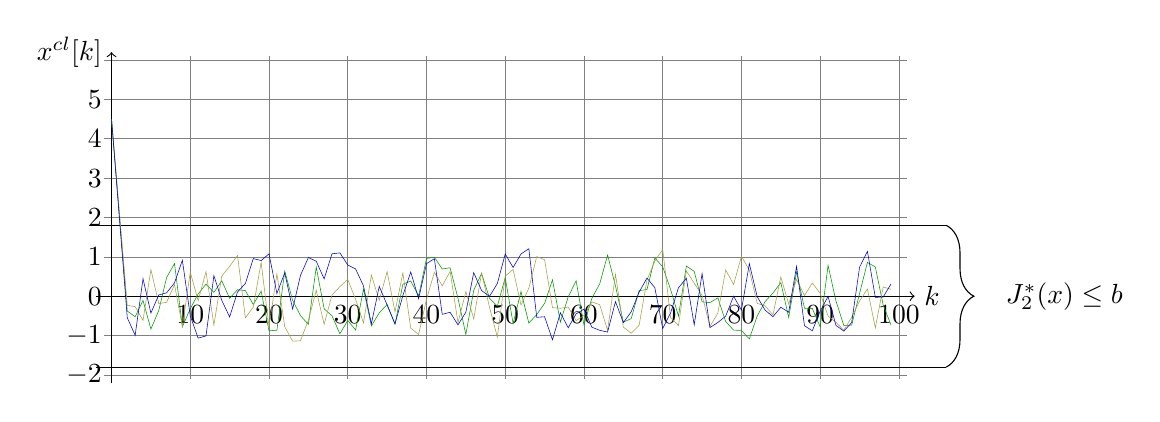
\begin{tikzpicture}[yscale = .5]
	\draw[very thin,color=gray] (-0.1,-2.1) grid (10.1,6.1);
    \foreach \x in {10,20,...,100} \draw (\x/10,0) node[below] {$\x$};
    \foreach \y in {-2,-1,...,5} \draw (0,\y) node[left] {$\y$};
    \draw (-.2,1.80102) -- (10.6,1.80102);
    \draw (-.2,-1.80102) -- (10.6,-1.80102);
    \draw [decorate,decoration={brace,amplitude=10pt},xshift=0pt,yshift=0pt] (10.6,1.80102) -- (10.6,-1.80102) node [midway,xshift=1.5cm] {$J_2^\ast(x)\leq b$};
    % \draw (-.2,4) -- (10.6,4);
    % \draw (-.2,-4) -- (10.6,-4);
    % \draw [decorate,decoration={brace,amplitude=10pt},xshift=0pt,yshift=0pt] (10.6,4) -- (10.6,-4) node [midway,xshift=1.5cm] {$x^{cl}[k]\in\mathcal \X^\infty_{\max}$};
    \draw[->] (-0.2,0) -- (10.2,0) node[right] {$k$};
    \draw[->] (0,-2.2) -- (0,6.2) node[left] {$x^{cl}[k]$};
	\draw[very thin,black!40!green] (0,4.5) -- (0.2,-0.37769) -- (0.3,-0.520842) -- (0.4,-0.108215) -- (0.5,-0.834513) -- (0.6,-0.362023) -- (0.7,0.476246) -- (0.8,0.829295) -- (0.9,-0.774026) -- (1.,-0.319506) -- (1.1,0.0565379) -- (1.2,0.30669) -- (1.3,0.0968538) -- (1.4,0.391411) -- (1.5,-0.0538486) -- (1.6,0.164445) -- (1.7,0.141598) -- (1.8,-0.212336) -- (1.9,0.126848) -- (2.,-0.877613) -- (2.1,-0.865174) -- (2.2,0.638466) -- (2.3,-0.106947) -- (2.4,-0.493973) -- (2.5,-0.718175) -- (2.6,0.738973) -- (2.7,-0.320137) -- (2.8,-0.497765) -- (2.9,-0.954995) -- (3.,-0.617526) -- (3.1,-0.859599) -- (3.2,0.181025) -- (3.3,-0.754288) -- (3.4,-0.424562) -- (3.5,-0.210048) -- (3.6,-0.709643) -- (3.7,0.305409) -- (3.8,0.385619) -- (3.9,0.00592743) -- (4.,0.958867) -- (4.1,0.988568) -- (4.2,0.691016) -- (4.3,0.722643) -- (4.4,-0.0545121) -- (4.5,-0.972004) -- (4.6,0.150141) -- (4.7,0.579977) -- (4.8,-0.051188) -- (4.9,-0.250251) -- (5.,0.4716) -- (5.1,-0.693329) -- (5.2,0.118012) -- (5.3,-0.682522) -- (5.4,-0.466949) -- (5.5,-0.18186) -- (5.6,0.417964) -- (5.7,-0.658329) -- (5.8,-0.0150836) -- (5.9,0.391728) -- (6.,-0.730995) -- (6.1,-0.0550463) -- (6.2,0.315063) -- (6.3,1.04568) -- (6.4,0.26213) -- (6.5,-0.659491) -- (6.6,-0.569369) -- (6.7,0.141955) -- (6.8,0.169819) -- (6.9,0.970814) -- (7.,0.746398) -- (7.1,0.17397) -- (7.2,-0.506768) -- (7.3,0.76502) -- (7.4,0.630173) -- (7.5,-0.144222) -- (7.6,-0.1625) -- (7.7,-0.0421583) -- (7.8,-0.644545) -- (7.9,-0.862389) -- (8.,-0.867818) -- (8.1,-1.08598) -- (8.2,-0.503064) -- (8.3,-0.138741) -- (8.4,0.0808979) -- (8.5,0.344021) -- (8.6,-0.53841) -- (8.7,0.617781) -- (8.8,-0.305312) -- (8.9,-0.312575) -- (9.,-0.779076) -- (9.1,0.782343) -- (9.2,-0.119298) -- (9.3,-0.743988) -- (9.4,-0.734647) -- (9.5,0.0728522) -- (9.6,0.859252) -- (9.7,0.742428) -- (9.8,-0.224105) -- (9.9,-0.73469);
	\draw[very thin,black!40!yellow] (0,4.5) -- (0.2,-0.233477) -- (0.3,-0.264914) -- (0.4,-0.61385) -- (0.5,0.676802) -- (0.6,-0.186819) -- (0.7,-0.155909) -- (0.8,0.294643) -- (0.9,-0.773144) -- (1.,0.612707) -- (1.1,-0.114674) -- (1.2,0.625243) -- (1.3,-0.733646) -- (1.4,0.510787) -- (1.5,0.757522) -- (1.6,1.03435) -- (1.7,-0.549086) -- (1.8,-0.278019) -- (1.9,0.85736) -- (2.,-0.777322) -- (2.1,0.568643) -- (2.2,-0.77823) -- (2.3,-1.14332) -- (2.4,-1.13117) -- (2.5,-0.607511) -- (2.6,0.149473) -- (2.7,-0.715438) -- (2.8,0.0289015) -- (2.9,0.242131) -- (3.,0.425234) -- (3.1,-0.0814754) -- (3.2,-0.679699) -- (3.3,0.538415) -- (3.4,-0.105062) -- (3.5,0.623901) -- (3.6,-0.395474) -- (3.7,0.588153) -- (3.8,-0.809184) -- (3.9,-0.97541) -- (4.,-0.0776675) -- (4.1,0.607461) -- (4.2,0.262878) -- (4.3,0.630362) -- (4.4,-0.674101) -- (4.5,0.118863) -- (4.6,-0.580474) -- (4.7,0.589902) -- (4.8,-0.281581) -- (4.9,-1.04013) -- (5.,0.508321) -- (5.1,0.679305) -- (5.2,-0.225995) -- (5.3,0.205712) -- (5.4,1.00673) -- (5.5,0.926658) -- (5.6,-0.291793) -- (5.7,-0.306287) -- (5.8,-0.276677) -- (5.9,-0.620541) -- (6.,-0.490798) -- (6.1,-0.146229) -- (6.2,-0.215277) -- (6.3,-0.869464) -- (6.4,0.558498) -- (6.5,-0.785469) -- (6.6,-0.941634) -- (6.7,-0.738693) -- (6.8,0.409311) -- (6.9,0.891481) -- (7.,1.1908) -- (7.1,-0.543656) -- (7.2,-0.746514) -- (7.3,0.64158) -- (7.4,0.329756) -- (7.5,0.022544) -- (7.6,-0.767645) -- (7.7,-0.430351) -- (7.8,0.667373) -- (7.9,0.295965) -- (8.,1.01241) -- (8.1,0.66112) -- (8.2,-0.18259) -- (8.3,-0.244123) -- (8.4,-0.475874) -- (8.5,0.488937) -- (8.6,-0.201315) -- (8.7,0.427962) -- (8.8,0.0128066) -- (8.9,0.334604) -- (9.,0.0719745) -- (9.1,-0.503969) -- (9.2,-0.662681) -- (9.3,-0.864852) -- (9.4,-0.532605) -- (9.5,-0.12178) -- (9.6,0.182521) -- (9.7,-0.804008) -- (9.8,0.235484) -- (9.9,0.173567);
	\draw[very thin,black!20!blue] (0,4.5) -- (0.2,-0.547731) -- (0.3,-0.993285) -- (0.4,0.443155) -- (0.5,-0.429577) -- (0.6,0.0322275) -- (0.7,0.0862037) -- (0.8,0.341086) -- (0.9,0.912223) -- (1.,-0.499284) -- (1.1,-1.06551) -- (1.2,-1.00807) -- (1.3,0.522486) -- (1.4,-0.105599) -- (1.5,-0.526862) -- (1.6,0.10804) -- (1.7,0.320731) -- (1.8,0.956571) -- (1.9,0.905223) -- (2.,1.0762) -- (2.1,0.0679059) -- (2.2,0.592277) -- (2.3,-0.326429) -- (2.4,0.53139) -- (2.5,0.982424) -- (2.6,0.888159) -- (2.7,0.439453) -- (2.8,1.07711) -- (2.9,1.10013) -- (3.,0.793551) -- (3.1,0.691838) -- (3.2,0.261129) -- (3.3,-0.700932) -- (3.4,0.250183) -- (3.5,-0.223874) -- (3.6,-0.701782) -- (3.7,0.0151031) -- (3.8,0.61661) -- (3.9,-0.0636195) -- (4.,0.82576) -- (4.1,0.951476) -- (4.2,-0.459941) -- (4.3,-0.408318) -- (4.4,-0.72846) -- (4.5,-0.407005) -- (4.6,0.598257) -- (4.7,0.144033) -- (4.8,-0.00489275) -- (4.9,0.322928) -- (5.,1.07148) -- (5.1,0.729876) -- (5.2,1.07207) -- (5.3,1.20548) -- (5.4,-0.537144) -- (5.5,-0.521942) -- (5.6,-1.10708) -- (5.7,-0.419542) -- (5.8,-0.801195) -- (5.9,-0.449948) -- (6.,-0.329329) -- (6.1,-0.786102) -- (6.2,-0.866297) -- (6.3,-0.91258) -- (6.4,-0.136829) -- (6.5,-0.670631) -- (6.6,-0.396601) -- (6.7,0.100334) -- (6.8,0.460408) -- (6.9,0.216292) -- (7.,-0.82042) -- (7.1,-0.425678) -- (7.2,0.213947) -- (7.3,0.456862) -- (7.4,-0.726849) -- (7.5,0.574493) -- (7.6,-0.796925) -- (7.7,-0.668417) -- (7.8,-0.504887) -- (7.9,-0.00101684) -- (8.,-0.352466) -- (8.1,0.826777) -- (8.2,-0.0117071) -- (8.3,-0.353103) -- (8.4,-0.521145) -- (8.5,-0.280625) -- (8.6,-0.408037) -- (8.7,0.758611) -- (8.8,-0.74968) -- (8.9,-0.878143) -- (9.,-0.376532) -- (9.1,-0.00501117) -- (9.2,-0.741025) -- (9.3,-0.886509) -- (9.4,-0.669708) -- (9.5,0.735438) -- (9.6,1.13667) -- (9.7,-0.0293156) -- (9.8,-0.0211713) -- (9.9,0.313614);
\end{tikzpicture}
\caption[Simulation Results for One Dimensional Example]{Three different closed-loop trajectories produced by the solution of~$(\exmp\ref{example:linesearch})$ for $x_0=4\frac{1}{2}$.
%
The level set~$J_2^\ast(x)\leq b$ which is invariant according to the input-to-state stability analysis.}
\label{figure:example:closed:loop:trajectories}
\end{figure}
\end{example}
